\RequirePackage[l2tabu, orthodox]{nag}

\documentclass[a4paper, 12pt, DIV=10, ngerman, abstracton, toc=bibliography, toc=listof]{scrreprt}

% compatibility
\usepackage{scrhack} % silences certain KOMA warnings
\usepackage{xltxtra} % fixes XeTeX stuff

% language support
\usepackage[ngerman]{babel}

% bibliography
\usepackage[backend=biber, style=alphabetic]{biblatex}
\bibliography{bibliography.bib}

% fonts
\defaultfontfeatures{Ligatures=TeX}
\setmainfont{Minion Pro}
\setsansfont{Myriad Pro}
\setmonofont{Consolas}
\urlstyle{same}

% line spacing
\usepackage{setspace} 
\setstretch{1.3}

% no paragraph indentation
\parskip 6pt
\parindent 0pt

% no widows
\usepackage[all]{nowidow}

\usepackage{xcolor}
\definecolor{lightgray}{gray}{0.96}

% listings
\usepackage{listings}
\lstset{
    basicstyle=\ttfamily\scriptsize,
    captionpos=b,
    frame=bt,
    numbers=left,
    numberstyle=\rmfamily\tiny\color{gray!50!black},
    keywordstyle=\bfseries,
    % backgroundcolor=\color{lightgray},
    stringstyle=\slshape,
    aboveskip=1cm,
    xleftmargin=8mm,
    framexleftmargin=8mm,
    aboveskip=1cm,
    showspaces=false,
    showtabs=false
}

\lstdefinelanguage{json}{
  morestring=[b]",
}

\lstdefinelanguage{pseudo}{
    keywords={var, foreach, in, function, return, end, do},
}

% referencing stuff
\usepackage[strict=true]{csquotes}
\PassOptionsToPackage{hyphens}{url}\usepackage{hyperref}
\usepackage{cleveref}
\usepackage[font=small,labelfont=bf]{caption}
\captionsetup{%
  figurewithin=chapter,
  tablewithin=chapter
}

% various extensions
\usepackage{siunitx} % numbers and units
\usepackage{booktabs} % good looking tables
\usepackage{dashrule} % dotted lines

% no warnings for underfull boxes in bibliography
\usepackage{etoolbox}
\apptocmd{\sloppy}{\hbadness 10000\relax}{}{}

% graphics directory
\graphicspath{{assets/}}

\begin{document}

\pagenumbering{roman}

% title page
\thispagestyle{plain}
\begin{titlepage}
\begin{center}
\includegraphics[width=5cm]{htwk_logo}\\
\vspace{0.3cm}
\normalsize
Fakultät für Informatik, Mathematik und Naturwissenschaften\\
\vspace{2.3cm}
\huge{\textbf{\textsf{Kookkurrenzbasierte Link Discovery am Beispiel von Produkttags}}}\\
\vspace{1cm}
\LARGE{\textsf{Masterarbeit}}\\
\vspace{2.3cm}
\normalsize
Sebastian Marr\\
mail@sebastianmarr.de\\
Leipzig, den 21. November 2013\\
\vspace{2.3cm}
Erstgutachter: Dr. Toralf Kirsten \\
Zweitgutachter: M.Sc. Martin Breest
\end{center}
\end{titlepage}

\begin{abstract}
Durch die Möglichkeit der Benutzerbeteiligung an der Beschreibung, Bewertung und Kategorisierung von Inhalten auf Online-Plattformen werden Begriffswelten aufgebaut, deren Auswertung großes Potenzial für die Verbesserung der Benutzererfahrung bietet. Diese Masterarbeit beschreibt ein Verfahren zum Finden von Zusammenhängen zwischen diesen Begriffen. Grundlage dafür stellen die Daten eines Tagging--Systems und die Ermittlung von Kookkurrenz dar. Die Begriffe und ihre Zusammenhänge werden in eine Graphenrepräsentation transformiert und durch Mining und Integration weiterer Datenquellen angereichert. Zur Priorisierung der Beziehungen für einen Anwendungsfall wird ein Verfahren mittels interaktiver evolutionärer Algorithmen vorstellt und angewendet. Die Ergebnisse der Erzeugung von Beziehungen und der Priorisierung werden präsentiert und schließlich die technische Umsetzung der genannten Verfahren beschrieben.
\end{abstract}
\chapter*{Erklärung}

Hiermit erkläre ich, dass die vorliegende Arbeit von mir selbstständig und nur unter Verwendung der aufgeführten Hilfsmittel erstellt wurde. Alle Stellen, die ich wörtlich oder sinngemäß aus veröffentlichten Schriften entnommen habe, wurden als solche gekennzeichnet. Diese Masterarbeit wurde weder als Ganzes noch in Auszügen für eine andere Prüfung angefertigt.

{
\vspace{32pt}
\noindent
\hdashrule{5cm}{1pt}{1pt 3pt}\\
Sebastian Marr\\
Leipzig, den 21. November 2013
}


\tableofcontents

\cleardoublepage

\pagenumbering{arabic}

\chapter{Einleitung}

Mit der steigenden Menge von nutzergenerierten Inhalten steigt auch die Menge von Metadaten, die mit diesen Inhalten verknüpft sind. Zur späteren Durchsuchbarkeit und Kategorisierung geben viele Online-Plattformen, Marktplätze und Online-Shops ihren Benutzern die Möglichkeit, Inhalte mit Metadaten zu versehen.

Eine oft genutzte Möglichkeit zur Beschreibung von Inhalten sind Tags. Dabei handelt es sich um Wörter oder Wortgruppen, die vom Benutzer frei gewählt werden können, um den Inhalt zu beschreiben. Dabei unterliegt die Eingabe von Tags möglichst wenigen Regeln, um dem Benutzer eine für ihn natürliche Beschreibung des Inhaltes zu ermöglichen. Dabei ist explizit, im Gegensatz zu einer Kategorisierung, die Vergabe von mehreren Tags vorgesehen.

Ein charakteristisches Merkmal von Tags ist dabei, dass sie nur einen bestimmten Aspekt des getaggten Objektes beschreiben. Dabei sind Tags nicht hierarchisch und es werden an keiner Stelle vom Nutzer explizite Zusammenhänge zwischen Tags erstellt. Jedoch liegt die Annahme, dass zwischen Tags Beziehungen herstellbar sind und sich mehrere Tags zu übergeordneten Themen zusammenfassen lassen, nahe. Der Benutzer berücksichtigt diese Beziehungen bei der Eingabe des Tags, formuliert sie jedoch nicht explizit. Die nachträgliche Rekonstruktion der Denkprozesse bei der Eingabe von Tags ist Thema dieser Arbeit.

Dabei ist zu beachten, dass Benutzer bei der Eingabe von Tags unterschiedliche Ziele verfolgen. Idealerweise werden Tags so vergeben, dass sie das getaggte Objekt inhaltlich beschreiben. Jedoch werden vom Benutzer bei der eingabe des Tags weitere Assoziationen hergestellt. Beispielsweise kann der Benutzer mit einem Objekt bestimmte Emotionen oder Wertungen verbinden, die sich in den vergebenen Tags wiederspiegeln.

Auf Marktplätzen, bei denen Verkäufern die Möglichkeit des Taggings ihre Produkte gegeben wird, besteht eine weitere Motivation in der Erhöhung der Auffindbarkeit des Produktes. Dabei kann die inhaltliche Qualität des Tags außer Acht gelassen werden, wenn bei Vergabe einer falschen Beschreibung die Sichtbarkeit des Produktes erhöht wird. Auch der Marktplatzbetreiber selbst kann so vorgehen, um zu versuchen, die Gesamtverkäufe zu steigern.

Die verschiedenen Motivationen der Benutzern von Tags erschwerden die nachträgliche Suche nach Assoziationen. Die vorliegende Masterarbeit beschäftigt sich mit Strategien zur Datenaufbereitung und Nutzung externer und interner Datenquellen und deren Integration mit Tag-Daten. Aus diesen Datenquellen wird eine Datenstruktur mit einem Kookurrenzgraphen als Basis aufgebaut und schließlich werden mit Hilfe von Clustering-Algrithmen daraus Themen extrahiert. Außerdem wird eine Evaluation der Ergebnisse und eine Analyse der verwendeten Methoden durchgeführt.

\section{Motivation und Anwendungen}

Die nachträgliche Herstellung von Assoziationen in vorhandenen Tag-Daten bietet einige Nutzungsmöglichkeiten für den Betreiber der Online-Plattform.

Die Beziehungen zwischen Tags können genutzt werden, um Suchergebnisse zu verbessern. Wenn zu einem Suchbegiff weitere relevante Begriffe bekannt sind, können diese im Suchergebnis mit enthalten sein um somit auch Objekte zu finden, die nicht direkt mit dem Suchbegriff getaggt sind. Außerdem können Suchen vom Benutzer mit Hilfe von verwandten Tags verfeinert werden.

Über die Zusammenfassung von Tags zu Themen lässt sich außerdem die Navigation einer Webseite verbessern. Aus den Themen lassen sich Kategorien oder Hierachien von Kategorien erzeugen, die besser den Denkmustern von Benutzern entsprechen. So sind auch Navigationskonzepte denkbar, die nicht hierarchisch, sondern assoziativ aufgebaut sind. Desweiteren können Tag-Assoziationen für Empfehlungssysteme genutzt werden, die einem Kunden zu einem bestimmten Artikel passende andere Artikel vorschlagen.

Im Bereich des Marketings können Beziehungen zwischen Tags genutzt werden, um für bestimmte externe Suchbegriffe spezielle Seiten zu erstellen (Landing Pages), die Inhalte zu diesem Suchbegriff bereitstellen oder Werbung für diese Suchbegriffe zu schalten. Außerdem können mit Hilfe des Kaufinteresses an bestimmten Themen über die Zeit Trends erkannt werden und mit entsprechenden Marketingmaßnahmen darauf reagiert werden.

All diese Anwendungen führen zu einer besseren Erfahrung für den Benutzer der Plattform. Die Präsentation von Daten kann besser auf die Denkmuster und Erwartungshaltungen des Benutzers angepasst werden. Dies führt in Konsequenz zu einem wirtschaftlichen Vorteil für den Plattformbetreiber.

\section{Kontext}

\section{Aufbau der Arbeit}
\chapter{Tagging--Systeme}
\label{tagging}

Das folgende Kapitel beschäftigt sich mit Tagging--Systemen. Dabei werden die Grundlagen, das Datenmodell und die Arten von Tagging--Systemen erläutert sowie das System von Spreadshirt, das in dieser Arbeit verwendet wurde, genauer erklärt. Dies umfasst die spezifischen Eigenschaften dieses Systems, die Diskussion der Datenqualität sowie das Mengengerüst der vorhandenen Daten.

\section{Grundlagen}
\label{tagging_basics}

\emph{Tags} sind eine Form von Metadaten, also ``Daten über Daten''. Sie erfüllen die Funktion der \emph{Beschreibung} von Dokumenten und werden im Allgemeinen von Benutzern angelegt. Dies steht im Gegensatz zu professionell kuratierten Metadaten wie beispielsweise Bibliothekskatalogen \cite{ma2004}.

Im Allgemeinen sind Tags kurze Schlagworte, die von dem Benutzer, der sie vergibt, frei gewählt werden können. Jedes Dokument kann mit beliebig vielen Tags versehen werden. Dies steht im Gegensatz zu einer festen, vorgegebenen Klassifikation mittels Kategoriebäumen, wie sie beispielsweise in E--Commerce--Systemen üblich sind, um Artikel zu ordnen. In solchen Kategoriebäumen kann ein Dokument üblicherweise nur in einer begrenzten Anzahl von Kategorien, meistens nur in einer, eingeordnet werden.

Die Menge der Tags eines Systems ist nicht hierarchisch geordnet und es bestehen keine explizit formulierten Beziehungen zwischen einzelnen Tags. Somit ergibt sich eine lose Kategorisierung der Dokumente, die, im Gegensatz zu formalen Taxonomien und Ontologien, ständig von den Benutzern erweitert und verändert wird \cite{sc2005}. \textcite{je2004} beschäftigt sich tiefer gehend mit dem Unterschied zwischen starrer Klassifikation und loser Kategorisierung.

Aus dieser Eigenschaft ergeben sich bestimmte Schwächen und Stärken von Tagging--Systemen, die von \textcite{ma2004} definiert wurden. Demnach liegen die Schwächen in der Mehrdeutigkeit von Tags und der mangelnden Kontrolle von Synonymen. Mehrdeutigkeit bezeichnet den Umstand, dass gleiche Tags zur Beschreibung von sehr unterschiedlichen Dokumenten genutzt werden können, da keine Systematik vorgegeben ist. Die mangelnde Kontrolle von Synonymen führt dazu, dass verschiedene Tags verwendet werden, um den gleichen Sachverhalt zu beschreiben.

Zu den von \textcite{ma2004} formulierten Stärken gehören die starke Ausrichtung von Tags an den Gedankengängen der Benutzer und dem einfacheren Durchstöbern von Dokumenten. Da die Tags von den Benutzern eines Systems formuliert werden, spiegeln sie deren Vokabular und deren Gedankengänge wieder. Werden Tags statt zum Finden von konkreten Dokumenten zum Durchstöbern genutzt, bieten sie größere Möglichkeiten, interessante Inhalte zu finden, als in einer starren Kategorisierung.

Tagging--Systeme enthalten demnach implizites Wissen, dass durch Data Mining extrahiert und genutzt werden kann. Im Rahmen dieser Arbeit wurden Tagging--Systeme als Ausgangspunkt für die Link Discovery mittels Kookkurrenz genutzt (siehe \cref{co-occurence,ld_tags}).

\subsection{Datenmodell von Tagging--Systemen}
\label{tagging_data}

Ein Tagging--System ist allgemein durch ein Tripel \(S=(D, T, U)\) von Mengen, sowie durch die Relation \(R = D \times U \times T\) definiert. 

\(D\) repräsentiert eine Menge von Dokumenten. Ein Dokument \(d\) kann ein beliebiger Datensatz sein, beispielsweise ein Design, Artikel oder Produkt. Die Menge \(U\) stellt alle Benutzer des Systems dar. Ein Benutzer \(u\) ist eine Entität mit beliebigen weiteren Attributen, die jedoch im Kontext des Tagging--Systems nicht weiter betrachtet werden. \(T\) repräsentiert die Menge der Tags. Ein Tag \(t\) ist eine Entität, die als benötigtes Attribut eine Zeichenkette besitzt, die zur Beschreibung von Dokumenten genutzt werden kann. \(T\) bildet das \emph{Vokabular} des Tagging--Systems.

Die Relation \(R\) beschreibt den Vorgang des \emph{Taggings}. Ein Benutzer \(u\) des Systems vergibt einen Tag \(t\) an ein Dokument \(d\), um den Inhalt von \(d\) mit der Zeichenkette von \(t\) zu beschreiben. Der Zeitpunkt der Vergabe des Tags wird durch einen Zeitstempel \(ts\) repräsentiert. \(R\) enthält demnach Quadrupel der Form \((d,t,u,ts)\).

\begin{figure}
\centering
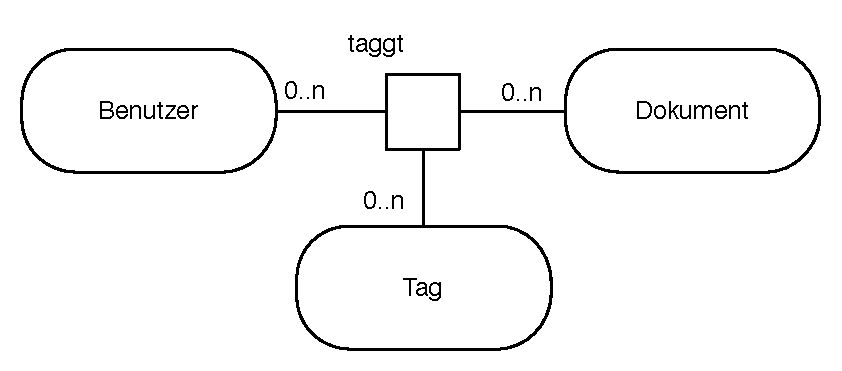
\includegraphics[width=0.75\textwidth]{tag_system}
\caption{FMC--Entity--Relationship--Diagramm eines Tagging--Systems}
\label{fig:tagging_erd}
\end{figure}

Das beschriebene Tagging--System lässt sich somit in ein Datenmodell mit den Entitätstypen \emph{Benutzer}, \emph{Dokument}, \emph{Tag} und  der ternären Beziehung \emph{Tagging} überführen. Dieses Modell ist in \cref{fig:tagging_erd} als Entity--Relationship--Diagramm dargestellt. Alle genannten Entitätstypen können weitere Attribute besitzen, die von der Anwendungsdomäne des konkret betrachteten Tagging--Systems abhängen.

\subsection{Arten von Tagging--Systemen}
\label{tagging_types}

Abhängig vom gewünschten Einsatzzweck des Tagging--Systems kann der Betreiber bestimmte Aspekte des Systems beschränken. Außerdem können die Benutzer einen vorherrschenden Umgang mit dem System entwickeln. Aus diesen Faktoren ergeben sich verschiedene Arten und Nutzungsmuster von Tagging-Systemen. Hauptsächlich kann zwischen offenen Tagging--Systemen, den so genannten \emph{Folksonomies} und den geschlossenen Tagging--Systemen unterschieden werden.

\subsubsection{Folksonomies}

Eine Folksonomy beschreibt ein weitestgehend offenes Tagging--System \cite{ma2004}. Bei dieser Art von System kann grundsätzlich jeder Benutzer jeden Tag an jedes Dokument vergeben. Außerdem stammen die Dokumente selbst meist ebenfalls von den Benutzern. Beispiele für Folksonomies sind der Bookmarking--Dienst \emph{Delicious} \cite{deli} und die Foto-Plattform \emph{Flickr} \cite{flickr}.

Der Begriff \emph{Folksonomy} steht im Gegensatz zur \emph{Taxonomie} und beschreibt den Umstand, dass die Kategorisierung und Ordnung von Inhalten vom \emph{folk}, also den Benutzern selbst vorgenommen werden \cite{vt2007}.

\subsubsection{Geschlossene Tagging--Systeme}

In geschlossenen Tagging--Systemen beschränkt der Betreiber des Systems bestimmte Aspekte. Dies können die Benutzer, die Tags vergeben dürfen, die Dokumente oder auch das Vokabular sein.

Eine häufige Form der Einschränkung, der auch das in dieser Arbeit verwendete System unterliegt (siehe \cref{tag_sprd}), ist die Einschränkung der Benutzer die ein Dokument taggen können. Oftmals ist dies nur den Autoren des Dokumentes selbst oder Benutzern mit besonderen Rechten, beispielsweise Moderatoren oder Angestellten des Betreibers, erlaubt.

In den meisten Tagging--Systemen stammen die Dokumente ebenfalls von den Benutzern des Systems, beispielsweise Artikel, Fotos oder Musikstücke. Jedoch kann die Erstellung der Dokumente eingeschränkt werden, wenn dies in der Anwendungsdomäne sinnvoll ist. Beispiele hierfür sind Produkte in Online--Shops. Diese werden nicht von den Benutzern erstellt, jedoch kann die Vergabe von Tags an diese einen Mehrwert liefern.

Die Einschränkung des Vokabulars kann vorgenommen werden, um Rechtschreibfehler und Fehleingaben der Tags zu vermeiden. Sie bringt jedoch den Nachteil mit sich, dass die Tags dann unter Umständen nicht mehr das Vokabular der Benutzer widerspiegeln und somit Inhalte für diese schwerer auffindbar sind.

\section{Tagging--System von Spreadshirt}

Nachdem im vorherigen Abschnitt die Grundlagen von Tagging--Systemen diskutiert wurden, beschäftigt sich dieser Abschnitt mit dem konkreten Tagging--Systems der Website \emph{Spreadshirt}, welches in dieser Arbeit für den initialen Schritt der Link Discovery genutzt wurde (siehe \cref{ld_tags}).

\subsection{Spreadshirt}
\label{spreadshirt}

Die vorliegende Masterarbeit wurde im Kontext der sprd.net AG (Spreadshirt) \cite{sprd2013} erstellt. Spreadshirt ist eine E--Commerce--Plattform, die es seinen Benutzern erlaubt, personalisierte Textilien und andere Artikel zu gestalten, zu kaufen und zum Verkauf anzubieten. Spreadshirt übernimmt die Produktion und den Versand der Produkte. Ein Produkt bezeichnet hierbei einen Produkttyp, beispielsweise ein T--Shirt, der mit einem oder mehreren Designs bedruckt wurde.

Das Erstellen von Designs und die Konfiguration eines Produktes, also das Positionieren von Designs auf Produkttypen, wird vollständig vom Benutzer durchgeführt. Es agieren grundsätzlich zwei Arten von Benutzern mit der Spreadshirt--Plattform: \emph{Kunden} und \emph{Partner}.

Als Kunden werden Benutzer bezeichnet, die Produkte bestellen. Diese Produkte können entweder von ihnen selbst oder von einem Partner erstellt worden sein. 

Partner sind Benutzer, die Designs oder Produkte erstellen und diese zum Verkauf anbieten. Zu diesem Zweck kann der Partner einen eigenen Shop auf der Spreadshirt--Plattform eröffnen. Kunden können in diesem Shop Produkte bestellen und der Partner erhält einen Anteil des Verkaufspreises, während Spreadshirt die Produktion und den Versand an den Kunden übernimmt.

Neben den von Kunden für sich selbst erstellten Produkten und den Partner--Shops existiert mit dem Spreadshirt--Marktplatz ein weiterer Vertriebskanal. Auf dem Marktplatz können Partner nach ihrer Zustimmung ihre Designs vertreiben. Kunden können nach Motiven suchen, die ihrem Geschmack entsprechen und diese bestellen, mit anderen Motiven kombinieren oder mit Texten versehen. Ein Produkt, das entweder in einem Partner--Shop oder auf dem Marktplatz positioniert und mit einem Preis versehen wurde, wird Artikel genannt.

\begin{figure}[t]
\centering
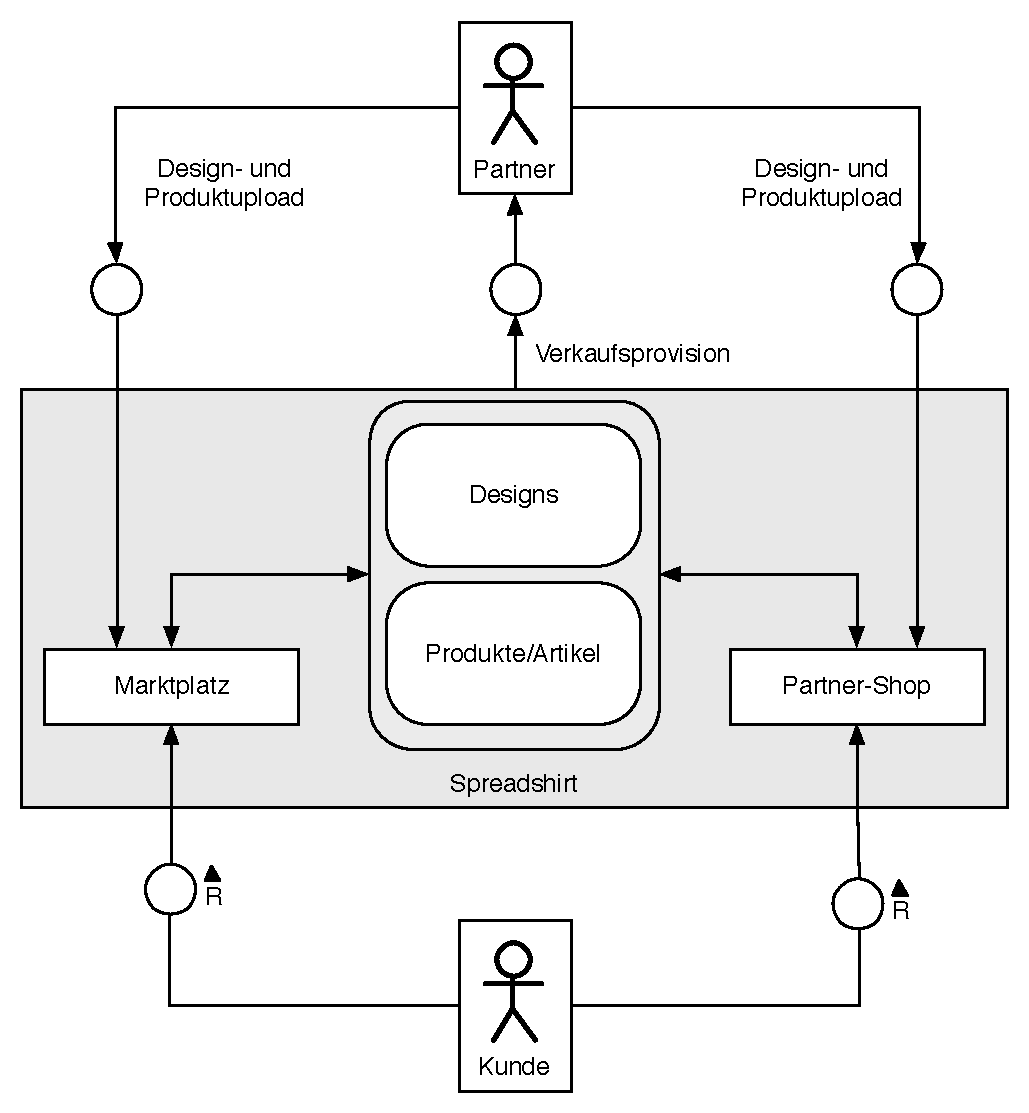
\includegraphics[width=0.65\textwidth]{how_spreadshirt_works}
\caption{FMC--Blockdiagramm der Spreadshirt--Bereiche und Benutzer}
\label{fig:howspreadshirtworks}
\end{figure}

Die grundsätzliche Funktionsweise der Spreadshirt--Plattform ist in \cref{fig:howspreadshirtworks} als FMC--Blockdiagramm dargestellt.

Das Suchergebnis für Suchen auf dem Marktplatz hängt maßgeblich von den Metadaten ab, die der Partner für seine Designs vergeben hat. Dazu gehören Tags, aber auch Titel und Beschreibung des Designs oder Produktes. In dieser Arbeit wird ausschließlich das Tagging--System betrachtet.

\label{platforms}
Spreadshirt betreibt aus historischen Gründen zwei Plattformen, deren Datenbestände größtenteils voneinander getrennt sind. Jeweils eine Plattform ist für den nordamerikanischen und den europäischen Markt zuständig. Im Kontext dieser Arbeit wird die europäische Plattform als Ausgangsbasis für alle Betrachtungen gewählt. Der Datenbestand dieser Plattform besteht aus circa 2 Millionen Tags, 6 Millionen Designs, 14 Millionen Produkten, 6 Millionen registrierten Nutzern und \num{750000} eröffneten Partner--Shops.

\subsection{Eigenschaften des Tagging--Systems}
\label{tag_sprd}

Im Fall von Spreadshirt ist die Vergabe von Tags auf die Menge der Partner \(P \subseteq U\) begrenzt (siehe auch \cref{spreadshirt}). Es handelt sich demnach um ein in \cref{tagging_types} beschriebenes geschlossenes Tagging--System.

Die Dokumente, die von den Partnern getaggt werden können, sind auf die Designs und Artikel beschränkt, die der Partner selbst angelegt hat. Eine Beschreibung kann somit ausschließlich durch den Autor des Inhaltes erfolgen. Deshalb fehlt im Vergleich zu anderen Tagging--Systemen auch die Information, welcher Benutzer den Tag vergeben hat, da diese implizit durch den Autor des Dokumentes gegeben ist.

Des Weiteren besitzen Tags in der Spreadshirt--Datenbank ein Attribut \emph{Sprache} aus der Menge \(L\). Die Sprache spielt bei der Eingabe und Anzeige der Tags zu Dokumenten eine Rolle. Je nach eingestellter Sprache auf der Website erstellt und sieht der Benutzer nur Tags, die mit dieser Sprache markiert sind.

Das Vokabular der Tags ist nicht eingeschränkt. Dies bringt zwangsläufig Probleme der Datenqualität mit sich, welche im folgenden Abschnitt erläutert werden.

\subsection{Datenqualität des Tagging--Systems}
\label{quality}

Die Qualität von Daten wird im Allgemeinen unter mehreren Gesichtspunkten beurteilt. Dazu gehören unter anderem \emph{Korrektheit}, \emph{Vollständigkeit}, und \emph{Redundanzfreiheit} \cite[S. 84 f.]{hkp2012}. Nachfolgend werden die bei Spreadshirt vorhandenen Tagging--Daten nach diesen Kriterien betrachtet und die Quellen eventueller Fehler \cite[S. 43 f.]{jo2003} diskutiert.

\subsubsection{Korrektheit}

Die Korrektheit der Tagging--Daten kann an vielen Punkten angezweifelt werden. Das hervorstechende Problem hierbei ist das Auftreten von Spam. Viele Partner versehen ihre Artikel und Designs mit Tags, die nicht den Inhalt beschreiben. Partner versehen ihre Designs und Artikel mit falschen Tags, damit diese bei populären Suchbegriffen gefunden werden.

Ein weiterer Defekt ist die Inkorrektheit des Attributes \emph{Sprache} der Tags. Die Sprache wird aus der Domain abgeleitet, die der Benutzer, der den Tag eingegeben hat, besucht hat. Viele Partner geben jedoch ihre Tags in mehreren Sprachen ein, um ihre Inhalte besser auffindbar zu machen. Dies führt in der Konsequenz dazu, dass das Attribut Sprache in einem nicht unwesentlichen Teil der Tags als falsch angesehen werden kann.

Die Quelle beider Fehler ist die bewusste Falscheingabe von Informationen, um einen persönlichen Vorteil zu erlangen, da die Partner versuchen, ihre Produkte möglichst zu vielen Sucheingaben in den Ergebnissen auftauchen zu lassen.
                                                                                                                                                                                                                                                                                                                                                                                                              
\subsubsection{Vollständigkeit}

Wie bereits in \cref{tag_sprd} beschrieben, fehlt in den Daten des Spreadshirt--Systems die Angabe, welcher Benutzer einen Tag vergeben hat. Außerdem besitzen die Taggings keinen Zeitstempel. Dies führt in der Konsequenz dazu, dass Spam schwerer erkannt werden kann. Zwar ist bekannt, wann ein Tag das erste Mal verwendet wurde, alle weiteren Verwendungen des Tags haben jedoch keinen Zeitstempel. Der Benutzer, der den Tag angelegt und verwendet hat, kann nur daraus abgeleitet werden, wer den getaggten Artikel angelegt hat.

Die Unvollständigkeit der Daten rührt in erster Linie daher, dass zum Zeitpunkt der Implementierung des Tagging--Systems noch nicht bedacht wurde, dass die fehlenden Attribute später nützlich sein können.

\subsubsection{Redundanzfreiheit}

Bedingt durch die Form der Dateneingabe besteht für das Vokabular des Tag--Systems ein großes Potential für redundante Daten. Da eingegebene Tags durch einen Separator getrennt eingegeben werden müssen, besteht hier Potential zur Fehleingabe. Wird der falsche Separator verwendet, werden die eigentlich getrennten Tags als eine einzige Entität abgespeichert.

Technisch kann jeder Tag genau ein Mal in der Datenbank vorkommen. Jedoch führen Tipp-- und Rechtschreibfehler, unterschiedliche Groß- und Kleinschreibung, verschiedene Arten zusammengesetzte Wörter zu schreiben, Leerräume vor, nach und zwischen Wörtern eines Tags und Tippfehler dazu, dass das gleiche Wort mehrfach in der Datenbank gespeichert wurde.

Außerdem führten in der Vergangenheit Systemfehler und Implementierungsfehler dazu, dass falsche, nicht druckbare Zeichen in den Tags enthalten waren. Nach Beseitigung der Fehler blieben die fehlerhaften Tags bestehen, so dass bei einer erneuten Eingabe des gleichen Wortes ein neuer Tag in der Datenbank angelegt wurde.

\subsection{Mengengerüst des Tagging--Systems}
\label{tag_amount}

Zum Zeitpunkt der Bearbeitung dieser Arbeit befanden sich im Datenbestand der europäischen Spreadshirt--Plattform:

\begin{itemize}
    \item \num{2072079} Tags in \num{15} verschiedenen Sprachen
    \item \num{6433410} Benutzer
    \item \num{26147860} Dokumente (\num{16494430} Artikel und \num{9653430} Designs)
    \item \num{71938905} Taggings
\end{itemize}

Diese Datenmengen stellen besondere Anforderungen an die Verarbeitung. Wie diese umgesetzt wurden, wird in \cref{system} diskutiert.

\section{Zusammenfassung}

Dieses Kapitel befasste sich mit Tagging--Systemen. Dazu wurden die Grundlagen und Begriffe genannt, die Vor-- und Nachteile von Tagging--System erläutert, das Datenmodell formalisiert und die grundsätzlichen Arten Folksonomy und geschlossenes Tagging--System unterschieden.

Außerdem wurde das im weiteren Verlauf dieser Arbeit verwendete Tagging--System von Spreadshirt \cite{sprd2013} näher betrachtet. Dazu wurden die speziellen Eigenschaften dieses Systems, die Datenqualität und die Menge der vorhandenen Daten beschrieben.

Das nachfolgende Kapitel beschäftigt sich mit dem zur Link Discovery angewandten Framework.
\include{ld_framework}
\chapter{Link--Discovery--Durchführung}
\label{link_discovery}

Das folgende Kapitel beschäftigt sich mit den im Rahmen dieser Arbeit unternommenen Schritten zur Link Discovery, also dem Finden von Beziehungen zwischen Wörtern und Wortgruppen. Dazu zählen die Erzeugung eines initalen Graphen aus den Daten Tagging--Systems, sowie dessen Anreicherung durch die Integration weiterer interner und externer Datenquellen.

\section{Initiale Erstellung aus Tagging--Daten}
\label{ld_tags}

Den Ausgangspunkt für den in \cref{ld_process} beschriebenen Prozess stellen die Daten des Tagging--Systems dar. Diese werden in \cref{tag_sprd} ausführlich beschrieben. Aus diesen Daten wird im ersten Schritt der Zielgraph erstellt, in welchen in allen weiteren Schritten weitere Daten integriert werden. Die in diesem Graph enthaltenen Knoten stellen ebenfalls die Kriterien für die Abfrage der weiteren Datenquellen dar.

Um den Ausgangsgraphen zu berechnen, sind die Schritte des Imports, der Bereinigung, der Reduktion, der Transformation und der Integration notwendig, welche im Folgenden genauer beschrieben werden.

\subsection{Import}

Die Daten liegen im Quellsystem, einer MySQL--Datenbank, in relationaler Form vor. Somit existieren Tabellen für die Tags, Dokumente und Verknüpfungen zwischen eben jenen. Da der Inhalt der Dokumente nicht relevant für die Link Discovery mittels Kookkurrenz sind, genügt es, die Tabellen der Tags und Verknüpfungen zu importieren.

Die Tags liegen in der Form \((i, s, l)\) vor, wobei \(i\) den eindeutigen Bezeichner des Tags, \(s\) die Zeichenkette und \(l\) die Sprache des Tags repräsentieren.

Die Verknüpfungen sind durch Tupel der Form \((i, t, d_t, d_i)\) repräsentiert, wobei \(i\) der eindeutige Bezeichner der Verknüpfung selbst ist. \(t\) ist der Bezeichner des Tags, \(d_t\) der Typ des Dokuments und \(d_i\) der Bezeichner des Dokumentes. \(d_t\) und \(d_i\) bilden also den zusammengesetzten Schlüssel des getaggten Dokumentes. 
 
\begin{figure}
\centering
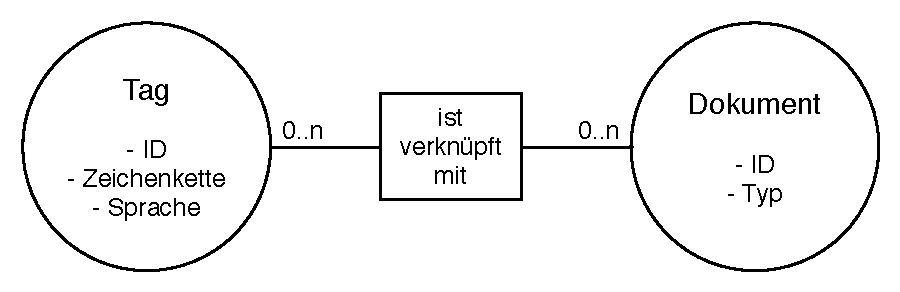
\includegraphics[width=0.6\textwidth]{tag_source_erd}
\caption{FMC--Entity--Relationship--Diagramm der Tagging--Quelldaten}
\label{fig:tag_source_erd}
\end{figure}

\begin{lstlisting}[language=json, label={lst:tag_import_tag}, caption={Beispiele für einen importierten Tag}]
{
    "_id" : ObjectId("51efc20147cae77dfc02e0ac"),
    "tag_id": 12345
    "tag": "segeln",
    "lang": "de"
}
\end{lstlisting}

\begin{lstlisting}[language=json, label={lst:tag_import_link}, caption={Beispiele für eine importierte Verknüpfung eines Tags mit einem Dokument}]
{
    "_id" : ObjectId("51efc20147cae77dfc02e0ac"),
    "object_id": 45678
    "object_type_id": 3,
    "tag_id": 12345
}
\end{lstlisting}

Die importierten Quelldaten sind beispielhaft in \cref{lst:tag_import_tag,lst:tag_import_link} dargestellt. Nach dem Import stehen \num{2072079} Tags und \num{71938905} Verknüpfungen zur Verfügung.

\subsection{Bereinigung}

An den Tagging--Daten liegen die in \cref{quality} genannten Defekte in Hinblick auf die Datenqualität vor. Diese sollten in einem Bereinigungsschritt reduziert werden. Hierbei liegt das Hauptaugenmerk auf der Erkennung von Duplikaten und später nicht verwertbaren Zeichenketten. Alle durchgeführten Maßnahmen zur Bereinigung beziehen sich hierbei auf die Eigenschaft \(s\) des Tags, also der Zeichenkette selbst.

In den unbereinigten importierten Daten existieren keine Duplikate in der Art, dass eine Paarung aus Zeichenkette und Sprache immer nur genau einmal in den Daten vorhanden ist. Jedoch enthalten viele der Tags nicht weiter verwertbare Zeichen wie nicht druckbare ASCII Zeichen, Anführungszeichen, Satzzeichen, Sonderzeichen sowie überflüssige Leerzeichen am Anfang und Ende der Zeichenkette. Außerdem existiert in den importierten Daten eine Unterscheidung zwischen Groß- und Kleinschreibung. Diese Unterscheidung bringt im Kontext der Link Discovery keine Vorteile und kann somit entfernt werden.

\begin{table}
\centering
% \arraystretch}{1.3}
\begin{tabular}{lcl}
    \toprule
    Rohdaten & \phantom{abc} & Bereinigte Daten \\
    \midrule
    \textbackslash u0003\textbackslash r\textbackslash nregenbogen && regenbogen \\
    RegenBogen && regenbogen \\
    "Regenbogen" && regenbogen \\
    regenbogen +einhorn && regenbogen einhorn\\
    \phantom{abc} regenbogen && regenbogen \\
    regenbogen && regenbogen \\
    \bottomrule
\end{tabular}
\caption{Beispiele für die Tag--Bereinigung}
\label{tab:tag_cleaning}
\end{table}

Somit besteht der Bereinigungsschritt darin, nicht verwertbare Zeichen zu entfernen und alle Großbuchstaben in Kleinbuchstaben umzuwandeln. Dadurch entstehen Duplikate, welche im darauf folgenden Reduktionsschritt zusammengeführt werden können. In \cref{tab:tag_cleaning} sind einige Beispiele für die Bereinigungen aufgeführt. Dabei ist gut zu erkennen, dass durch die Bereinigungen Duplikate erzeugt werden.

\subsection{Reduktion}

Der Reduktionsschritt dient zur Einschränkung der Gesamtdaten auf eine nützliche oder handhabbare Menge. Außerdem kann durch Reduktion auch die Datenqualität verbessert werden.

Im Fall der Tagging--Daten liegt das Hauptaugenmerk im Reduktionsschritt auf der Entfernung von Duplikaten, die bei der Bereinigung entstanden sind. Gleichzeitig muss sicher gestellt werden, dass keine Informationen über die Verwendung der Tags verloren gehen. Somit besteht die Duplikatentfernung der Tags im Zusammenführen von Datensätzen mit gleichen Zeichenketten und Sprachen. Gleichzeitig werden auch die Verwendungen der Tags zusammengeführt.

Werden die Verknüpfungen zweier Tags mit Dokumenten zusammengeführt, können auch dabei wieder Duplikate entstehen. Diese müssen in diesem Fall entfernt werden, da ein Tag nicht mehrmals mit einem Dokument verknüpft werden kann. Das Zusammenführen von Tags ist exemplarisch in \cref{fig:tag_reduction} dargestellt.

\begin{figure}
\centering
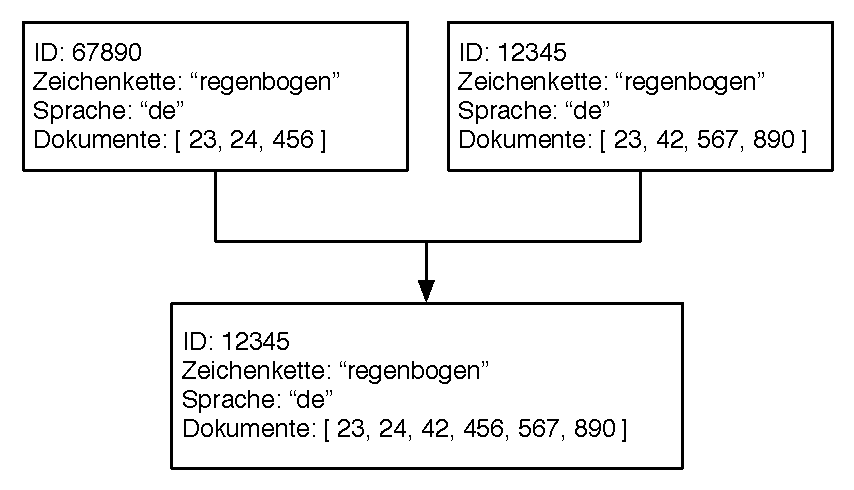
\includegraphics[width=0.7\textwidth]{tag_reduction}
\caption{Beispiel für das Zusammenführen der bereinigten Tags}
\label{fig:tag_reduction}
\end{figure}

Dabei findet ebenfalls eine Denormalisierung der Daten statt, da alle Dokumente, für die ein Tag vergeben werden, direkt mit in das Tag--Dokument gespeichert werden. Dies ist beispielhaft in \cref{lst:tag_denormalization} abgebildet. Das Attribut \emph{links} enthält alle Verknüpfungen des Tags mit Dokumenten.

\begin{lstlisting}[language=json, label={lst:tag_denormalization}, caption={Denormalisierte Tag-Daten}]
{
    "_id" : ObjectId("51efc20147cae77dfc02e0ac"),
    "string": "segeln"
    "language": "de",
    "links": [
        {
            object_id: 45678, 
            object_type_id: 3
        },
        {
            object_id: 98764, 
            object_type_id: 4
        },
        ...
    ]
}
\end{lstlisting}

Eine weitere im Rahmen dieser Arbeit unternommene Maßnahme zur Datenreduktion bestand darin, sich auf die Menge der Tags zu beschränken, deren Attribut \(l\) den Wert \emph{de} besitzt. Praktisch handelt es sich um alle Tags, die als deutsch gekennzeichnet in der Datenbank gespeichert sind. Diese Einschränkung wurde vorgenommen, um die zu verarbeitende Datenmenge überschaubar zu halten. Außerdem wird dadurch der nationale Kontext, in dem die Begriffe verwendet wurden, weitestgehend beibehalten.

Ein letzter Reduktionsschritt besteht in der Entfernung der Tags, deren Zeichenketten eine Länge von \num{1} besitzen, da in der deutschen Sprache keine einbuchstabigen Wörter existieren.

Nach der beschriebenen Reduktion befinden sich noch \num{314351} Tags und \num{23255714} Verknüpfungen in der Datenbank. Dies entspricht einer Reduktion von ca. \num{68} Prozent gegenüber der importierten Menge von Objekten.

\subsection{Transformation}

Der Transformationsschritt beschreibt die Überführung der Daten in die Form, die für das Ergebnis benötigt wird. Im Falle der Tagging--Daten bedeutet dies eine Umformung in die Form des Kookkurrenzgraphen, also die Erzeugung von Knoten- und Kantenobjekten. Die Umsetzung dieser Transformation mittels des Programmiermodelles MapReduce wurde in \cref{mapreduce_cooccurence} genauer beschrieben.

Je Tag wird ein Datenbankdokument erzeugt, dass den Knoten repräsentiert. Dieses besitzt als Attribute zum einen die Zeichenkette und die Sprache des Tags, aus dem es erzeugt wurde. Zum anderen wird ein Unterdokument hinzugefügt, welches weitere Eigenschaften des Ausgangstags beschreibt. Dies umfasst die Anzahl der Verwendungen und die eindeutigen Bezeichner der Dokumente, also Artikel oder Designs, die mit dem Tag getaggt wurden. Außerdem wird im Transformationsschritt für jeden Knoten ein global eindeutiger Bezeichner erzeugt, um das spätere Referenzieren der Knoten einfacher zu machen. Zeichenkette und Sprache des Knotens stellen einen zusammengesetzten Schlüssel dar und sind in der Knotenmenge eindeutig. \cref{lst:tag_transform_node} zeigt ein Beispiel für ein in der Datenbank abgelegtes Knotendokument.

\begin{lstlisting}[language=json, label={lst:tag_transform_node}, caption={Tag--Knoten als JSON--Dokument}]
{
    "_id" : ObjectId("51efc20147cae77dfc02e0ac"),
    "language" : "de",
    "string" : "mama",
    "tagProperties" : {
        "occurenceCount" : 3,
        "articleCount" : 2,
        "designCount" : 1,
        "articleIDs" : [
            24231101,
            24231105
        ],
        "designIDs" : [
            15514592
        ]
    }
}
\end{lstlisting}

Die Erzeugung der Kanten erfolgt wie in \cref{mapreduce_cooccurence} beschrieben. Für  jedes gemeinsame Auftreten von zwei Tags werden zwei Datenbankdokumente erzeugt. Dieses beschreiben gerichtete Kanten zwischen den Tags, die ein gemeinsames Auftreten der Tags repräsentieren. Neben Quell- und Zielknoten enthält eine Kante den Kantentyp sowie weitere Informationen über die Art der Verbindung. Im Fall von Kookkurrenzkanten ist dies zum einen die absolute Anzahl gemeinsamer Vorkommen der Tags, zum anderen die in \cref{measures} beschriebenen Kookkurrenzmaße. Der Kantentyp ist aus der Berechnung folgend der Typ der Tag--Kookkurrenz. Ein Beispiel JSON--Dokument für eine Kante ist in \cref{lst:tag_transform_edge} zu sehen.

\begin{lstlisting}[language=json, label={lst:tag_transform_edge}, caption={Tag--Kante als JSON--Dokument}]
{
    "_id" : ObjectId("51efd6f61177ff360605bd99"),
    "source" : ObjectId("51efc1af47cae77dfc00c3f8"),
    "target" : ObjectId("51efc1e047cae77dfc02087c"),
    "type" : "tag-co-occurence",
    "occurences" : 1,
    "dice" : 0.0001317089232795522,
    "jaccard" : 0.00006585879873551106,
    "cosine" : 0.008115343414514944
}
\end{lstlisting}

\subsection{Integration}

Da der aus den Tagging--Daten generierte Kookkurrenzgraph die Ausgangsbasis für alle weiteren Operationen darstellt, muss im Sinne der Integration nichts getan werden. Die transformierten Daten müssen lediglich in die Zieldatenbank kopiert werden.

Durch die Schritte, die zur Link Discovery aus den Tagging--Daten verwendet wurden, wurden insgesamt \num{314351} Knoten und \num{21834868} Kanten erzeugt, welche nun durch weitere Schritte angereichert werden sollen.

\subsection{Ergebnisse}

\section{Anreicherung mit Clicktracking-Daten}
\label{clicktracking}

Spreadshirt betreibt ein Clicktracking--System, welches die Klicks der Benutzer auf Artikel und Designs auf Suchergebnisseiten aufzeichnet. Dabei ist unerheblich, ob der Benutzer bei Spreadshirt registriert und angemeldet ist. Dieses System sammelt Daten von beiden Spreadshirt--Plattformen (siehe \cref{platforms}). In \cref{fig:search_result} ist beispielhaft eine Suchergebnisseite der Spreadshirt--Plattform abgebildet, welches die gefundenen Designs für eine Suchanfrage auflistet.

\begin{figure}
\centering
\includegraphics[scale=0.25]{search_result}
\caption{Suchergebnisseite}
\label{fig:search_result}
\end{figure}

Die von diesem System erzeugten Daten können für die Link Discovery von großer Bedeutung sein, da sie eine andere Perspektive auf die Begriffe im Graphen liefern. Die Tags liefern die Sicht der Partner, also der Personen, die Inhalte hochladen und verkaufen möchten. Die Klicks beschreiben die Sicht der Käufer, also der Personen, die nach Inhalten suchen. Durch die Auswertung der Clicktracking--Daten ergibt sich also die Möglichkeit, eine Form der Validierung der durch Partner vergebenen Metadaten zu erhalten. Die Annahme hierbei ist, dass Käufer nur auf Suchergebnisse klicken, die eine inhaltliche Relevanz zum eingegebenen Suchbegriff besitzen und somit ihren Erwartungen bezüglich des Suchbegriffes gerecht werden.

Wie bereits für die Tagging--Daten, werden im Folgenden auch für das Clicktracking die Schritte Import, Bereinigung, Reduktion, Transformation und Integration näher erläutert. Der Ansatz zur Erzeugung der Verbindungen ist ebenfalls kookkurrenzbasiert.

\subsection{Import}
\label{click_import}

Das Clicktracking--System erzeugt Dateien im JSON--Format, die zu jedem Klick auf einer Ergebnisseite die wesentlichen Informationen enthalten. Pro Klick ist ein JSON--Dokument in den Dateien abgespeichert. Ein Beispiel für ein solches Dokument ist in \cref{lst:click_raw} dargestellt.

\begin{lstlisting}[language=json, label={lst:click_raw}, caption={Clicktracking - Rohdokument als JSON}]
{
    "date": "01.07.2013 00:09:31_633",
    "path": "/track/eu/205909/1E3B6E3E-4496-C51A14A8FA25/2.10.4/list",
    "params": {
        "locale": "[de_DE]",
        "search-query": "[biene]",
        "cl": "[a18869874, p25446183, i49]"
    }
}
\end{lstlisting}

Ein Clicktracking--Dokument enthält die Attribute \emph{Datum}, \emph{Pfad}, \emph{Gebietsschema}, \emph{Suchbegriff} und die Daten des eigentlichen Klicks, also den geklickten \emph{Artikel}, das geklickte \emph{Produkt} und den \emph{Index}, also die Position des geklickten Inhaltes auf der Suchergebnisseite. Die Unterscheidung zwischen Produkt und Artikel ist im Domänenmodell von Spreadshirt begründet (siehe auch \cref{spreadshirt} und für die Link Discovery nicht von Interesse. Es genügt, den geklickten Artikel im Weiteren näher zu betrachten.

Auffällig ist, dass die Möglichkeiten des JSON--Formates bei der Speicherung der Klickdaten nicht vollständig ausgenutzt wurden. So sind die Werte, die das geklickte Dokument beschreiben, als Zeichenkette abgelegt und zusätzlich die eindeutigen Bezeichner mit einem Buchstaben versehen, der ihren Typ angibt. Des weiteren enthalten  das Gebietsschema und der Suchbegriff zusätzliche eckige Klammern. Diese Defekte sollten im Bereinigungsschritt beseitigt werden, um ein nutzbareres Datenformat zu erhalten.

Da das Clicktracking--System zum Zeitpunkt des Imports erst 3 Monate Daten aufzeichnete, standen \num{2249942} solcher Klickdokumente zur Verfügung.

\subsection{Bereinigung}

Im Bereinigungsschritt müssen zunächst die genannten Defekte der Klickdaten beseitigt werden. Dazu gehört die Entfernung der eckigen Klammern in Suchbegriff und Gebietsschema und die Extraktion des eindeutigen Bezeichners des geklickten Artikels. Aus dem Gebietsschema ist nur die Sprache von Interesse. Außerdem wurden für den Suchbegriff die gleichen Bereinigungsoperationen wie für die Tagging--Daten vorgenommen, also die Entfernung von überflüssigen Leerzeichen, Groß-/Kleinschreibung, nicht druckbarer Sonderzeichen und Satzzeichen.

Im Bereinigungsschritt werden so auch einfacher verarbeitbare Dokumente erzeugt, da die Möglichkeiten des JSON--Formates besser ausgenutzt werden. \cref{lst:tag_cleanup} zeigt das Ergebnis der Bereinigung des in \cref{click_import} gezeigten Beispieldokumentes.

\begin{lstlisting}[language=json, label={lst:tag_cleanup}, caption={Bereinigtes Clicktracking--Dokument}]
{
    "_id": ObjectId("51e7b1e0417498f9c6868939"),
    "query" : "biene",
    "date" : "2013-07-01T00:09:31.633Z",
    "articleId" : 18869874,
    "index" : 57,
    "language" : "de"
}
\end{lstlisting}

\subsection{Reduktion}

Die Reduktion der Clicktracking--Daten besteht zum einen aus einer Duplikatentfernung, zum anderen aus der Einschränkung der Sprache.

Im Sinne der Kookkurrenz ist es nicht von Bedeutung, wenn Paare aus Suchbegriffen und geklickten Artikeln mehrfach auftauchen, da hierfür nur das gemeinsame Auftreten unterschiedlicher Suchbegriffe betrachtet wird. Somit besteht die Duplikatentfernung lediglich darin, aus mehrfach vorkommenden Artikel-/Klickpaaren genau eines auszuwählen.

Außerdem erfolgte, wie schon bei den Tag--Daten, eine Einschränkung auf Klicks, die als \emph{deutsch} gekennzeichnet sind.

Nach dem Reduktionsschritt verblieben zur Transformation noch \num{411341} Klicks.

\subsection{Transformation}

Im Transformationsschritt wird für die Clicktracking--Daten ein Kookkurrenzgraph berechnet. Die Kookkurrenz bestimmt sich hierbei daraus, welche Suchbegriffe zum Klick auf einen Artikel geführt haben. Wird ein Artikel zu mehreren Suchbegriffen geklickt, liegt die Vermutung nah, dass zwischen den Suchbegriffen ein irgendwie gearteter Zusammenhang besteht.

Ziel der Transformation ist somit die Erzeugung von Knoten und Kanten. Die Knoten besitzen zusätzliche Eigenschaften, die die Eigenschaften des durch den Knoten repräsentierten Begriffes im Kontext des Clicktrackings widerspiegeln. Konkret sind dies die Artikel, die zu dem Begriff als Suchbegriff geklickt wurden. \cref{lst:click_node} zeigt beispielhaft ein erzeugtes Knotendokument.

\begin{lstlisting}[language=json, label={lst:click_node}, caption={Knotendokument mit Clicktracking--Eigenschaften}]
{
    "_id": ObjectId("51e7f1e04146498f9c6868945"),
    "string": "biene",
    "language": "de",
    "clickProperties": [
        { "articleId": 4512 },
        { "articleId": 4794 },
        ...
    ]
}
\end{lstlisting}

Die Kanten besitzen die gleiche Form wie die Kookkurrenzkanten, die bei der Integration der Tagging--Daten erzeugt wurden. Ein Beispiel für ein solches Kantendokument ist in \cref{lst:click_edge} dargestellt.

\begin{lstlisting}[language=json, label={lst:click_edge}, caption={Clicktracking--Kookkurrenzkante}]
{
    "_id": ObjectId("51e91aff3b6a20bfd68c468a")
    "source" : ObjectId("51e91af93b6a20bfd68b0bed"),
    "target" : ObjectId("51e91aff3b6a20bfd68c463e"),
    "type": "tag-co-occurence",
    "occs" : 1,
    "dice" : 0.003883495145631068,
    "jaccard" : 0.0019455252918287938,
    "cosine" : 0.04410810913912309
}
\end{lstlisting}

Die Durchführung des Transformationsschrittes erfolgte ebenfalls mittels MapReduce (siehe \cref{mapreduce_cooccurence}). Dadurch wurden \num{92727} Knoten und \num{310860} Kanten erzeugt.

\subsection{Integration}
\label{click_integration}

Die Integration der erzeugten Daten stellt eine Vereinigung des vorhandenen Zielgraphen mit dem im Transformationsschritt erzeugten Kookkurrenzgraphen dar.

Die Knotenmenge wird derart vereinigt, dass die Knotenmenge des Zielgraphen die Eigenschaft behält, dass Paare aus Sprache und Zeichenkette eindeutig sind. Somit werden bei bereits vorhandenen Knoten die zusätzlichen Informationen bezüglich des Clicktrackings als Attribute hinzugefügt. Existiert eine Kombination aus Sprache und Zeichenkette noch nicht im Zielgraph, so wird der entsprechende Knoten kopiert.

Da die erzeugten Kanten einen noch nicht im Graph vorhandenen Typ besitzen, müssen keine Kanten zusammengeführt werden. Jedoch werden die Bezeichner der Ziel- und Quellknoten entsprechend angepasst, wenn bei der Integration der Knoten eine Zusammenführung stattgefunden hat.

Durch dieses Vorgehen konnten der Knotenmenge \num{78237} Knoten, und somit auch neue Begriffe hinzugefügt werden. Die Kantenmenge wurde, wie bereits erläutert, um \num{310860} Kanten erweitert.

\subsection{Ergebnisse}

\section{Anreicherung durch Zerlegung von Wortgruppen}
\label{decomposition}

Die Zerlegung von Tags, die aus mehr als einem Wort bestehen, stellt zwar keine Integration anderer Datenquellen dar, kann aber trotzdem zum Auffinden neuer Verknüpfungen nützlich sein. Außerdem kann es für weitere Integrationsschritte von Nutzen sein, möglichst viele Einzelwörter im Datenbestand zu haben (siehe \cref{wortschatz}).

Zum Zeitpunkt des Importes befanden sich \num{147364} Tags in der Datenbank, die aus mehreren Wörtern bestehen. Dies entspricht \num{47} Prozent aller bereinigten deutschen Tags. Dieser Umstand legt die Vermutung nahe, dass in diesen zusammengesetzten Tags auch Wörter enthalten sind, die nicht als Einzelwörter existieren.

Werden diese Tags in ihre Einzelwörter zerlegt, entstehen einerseits unter Umständen neue Knoten, andererseits können in diesem Schritt Kanten vom Typ \emph{Zerlegung} beziehungsweise \emph{Zusammensetzung} eingefügt werden. Somit sind nach dem Schritt der Zerlegung weitere Informationen über den Kontext, in dem Wörter verwendet werden, verfügbar. \cref{fig:decomposition} zeigt beispielhaft das Ergebnis einer solchen Zerlegung.

Durch die Anwendung des Zerlegungsschrittes auf die vorhandenen Begriffe aus den Tagging-Daten wurden insgesamt \num{38349} Knoten und \num{1238900} Kanten erzeugt, die für spätere Analyseschritte genutzt werden können.

\begin{figure}
\centering
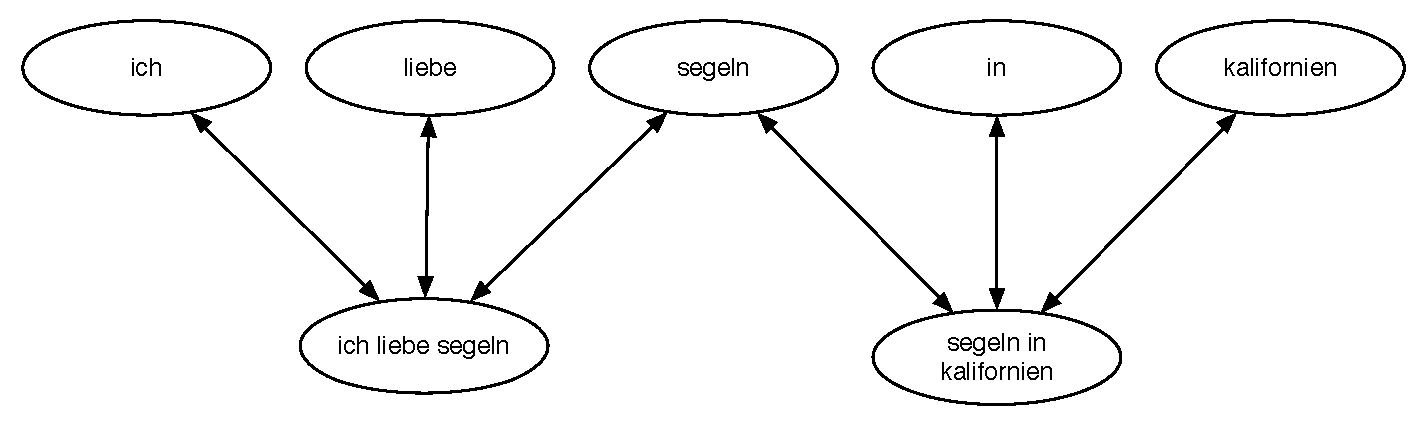
\includegraphics[width=\textwidth]{decomposition}
\caption{Beispielhafter Graphausschnitt nach der Zerlegung}
\label{fig:decomposition}
\end{figure}

\subsection{Vorgehensweise}

\subsection{Ergebnisse}

\section{Anreicherung mit Wortschatz-Daten}
\label{wortschatz}

Wie in \cref{used_sources} bereits einführend beschrieben, betreibt ein Wortschatz--Projekt \cite{ws2013}. Im Rahmen dieses Projektes wird durch die Analyse von großen Textmengen eine Datenbank deutscher Wörter, deren Bedeutungen, grammatikalische Eigenschaften, Häufigkeiten und Kookkurrenzen in Texten und Beziehungen zu anderen Wörtern aufgebaut. Somit stellt dieses Projekt eine sehr gute Möglichkeit dar, weitere Beziehungen zwischen den schon im Graph vorhandenen Knoten herzustellen. Neben den Daten, die im Spreadshirt--Kontext entstehen, können somit auch allgemeine lexikalische Daten hinzugefügt und für spätere Analysen genutzt werden.

Neben dem Webportal stellt dieses Projekt eine API bereit, über die die Daten des Wortschatzes programmatisch abgefragt werden können. Diese API wurde mittels einer Bibliothek für die Programmiersprache Ruby \cite{wlapi2013} im Rahmen dieser Arbeit für einen weiteren Integrationsschritt zur Link Discovery genutzt. Dazu wurden die Informationen \emph{Grundform}, \emph{Wortformen}, \emph{Kategorien}, \emph{Synonyme} und \emph{Thesaurus--Beziehungen} ausgewertet.

Wie bereits für die anderen Datenquellen, werden im Folgenden auch für den Wortschatz die Schritte des Imports, der Bereinigung, der Reduktion, der Transformation und der Integration beschrieben.

\subsection{Import}

Da für die Anfrage an die Wortschatz--API nur Einzelwörter und keine Wortgruppen genutzt werden können, muss eine Auswahl der anzufragenden Daten getroffen werden. Im Rahmen dieser Arbeit wurden alle Einzelwörter, die zum Zeitpunkt des Importes der Wortschatz--API zur Verfügung standen, ausgewählt. Dabei handelt es sich um \num{197614} einzelne Wörter. Da die Daten in der Datenbank zu diesem Zeitpunkt keine Groß- und Kleinschreibung enthielten, die Wortschatz--API diese jedoch berücksichtigt, wurde jedes Wort jeweils groß und klein geschrieben angefragt. Somit wurde die doppelte Menge an Datensätzen, \num{395228} Dokumente, erzeugt.

Die Ergebnisse wurden mittels eines Ruby--Skriptes in MongoDB importiert. Dabei wurde je angefragtem Wort ein Dokument erzeugt, dass die Informationen des Wortschatzes über dieses Wort enthält. Eines dieser Dokumente ist zu Illustrationszwecken in \cref{lst:wortschatz_import} dargestellt. Das Feld \emph{baseform} enthält die Grundform des Wortes mit der Wortart und \emph{domain} die Kategorien des Wortes.

\begin{lstlisting}[language=json, label={lst:wortschatz_import}, caption={Wortschatz--Dokument nach dem Import}]
{
    "_id" : ObjectId("51f7aa06eba16044e900015a"),
    "string" : "Kopf",
    "baseform" : [ 
        "Kopf", 
        "N"
    ],
    "domain" : [ 
        "Medizin", 
        "Anatomie", 
        "Literarische/Motive/Stoffe/Gestalten", 
        "Körperteile"
    ],
    "synonyms" : [  
        "Chef", 
        "Figur", 
        "Gestalt", 
        "Haupt", 
        "Jemand", 
        "Individuum", 
        "Figur"
    ],
    "thesaurus" : [ 
        "Titel", 
        "Hand", 
        "Kopf", 
        "Mensch", 
        "Gesicht", 
        "Spitze", 
        "Arm", 
        "Gestalt"
    ],
    "wordforms" : [ 
        "Kopf", 
        "Köpfe", 
        "Köpfen", 
        "Kopfes", 
        "Kopfs"
    ]
}
\end{lstlisting}

Hierbei ist zu beachten, dass nicht alle Attribute bei allen Wörtern vorhanden sind. Dies hängt davon ab, ob der Wortschatz die Informationen zur Verfügung stellen kann. Somit ist es auch möglich, dass Dokumente erzeugt werden, die keine zusätzlichen Informationen enthalten.

\subsection{Bereinigung}

Zur Bereinigung der importierten Wortschatz--Daten muss in einem ersten Schritt die Groß- und Kleinschreibung entfernt werden, da diese an erster Stelle nur für die Anfragen an die API wieder in den Datenbestand eingeführt wurde.

Weiterhin werden die Kategorien ``Vorname'' und ``Nachname'' entfernt, da diese an über \num{25000} Wörter vergeben sind und somit für die Verwendung zur Link Discovery ungeeignet sind und zu viele irrelevante Kanten erzeugen würden.

Ein letzter Bereinigungsschritt besteht in der Veränderung des Formates der Grundform des Wortes. Die Wortschatz--API liefert lediglich ein Array, in dem das erste Element die Grundform und das zweite Element die Wortart ist. Zur Bereinigung wird diese Eigenschaft in ein geeignetes JSON--Format überführt, welches in \cref{lst:word_baseform} dargestellt ist.

\begin{lstlisting}[language=json, label={lst:word_baseform}, caption={Grundform eines Wortes}]
{
    _id: ...,
    string: "Kopfs",
    baseform: {
        word: "Kopf",
        type: "N"
    }
}
\end{lstlisting}

\subsection{Reduktion}

Der Reduktionsschritt besteht in der Zusammenführung von Dokumenten mit gleichen Wörtern, welche im Bereinigungsschritt entstanden sind. Wie schon bei der Reduktion der Tagging--Daten, muss auch hierbei das Entstehen neuer Duplikate vermieden werden. Dies bedeutet, dass die gefundenen Wortbeziehungen ebenfalls zusammengeführt werden, wobei jedes verbundene Wort nur einmal enthalten sein darf. Die Reduktion ist beispielhaft in \cref{fig:wortschatz_reduction} dargestellt. Dabei ist zu beachten, dass bei der Zusammenführung mehrere Grundformen entstehen können, wodurch dieses Attribut in ein Array umgewandelt wird.

\begin{figure}
\centering
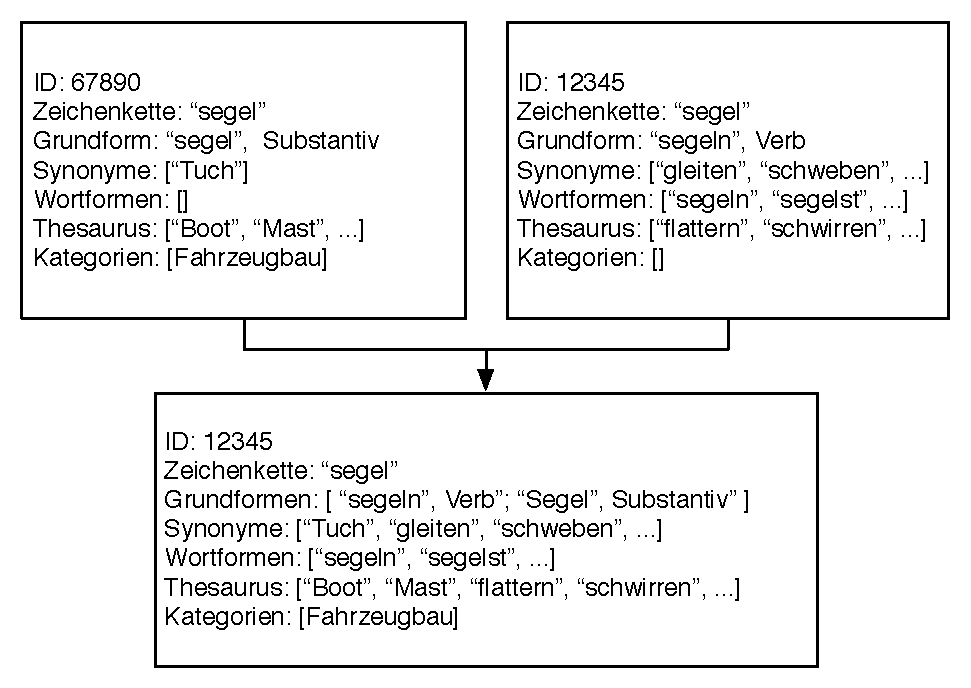
\includegraphics[width=0.8\textwidth]{wortschatz_reduction}
\caption{Reduktion der Wortschatz--Daten}
\label{fig:wortschatz_reduction}
\end{figure}

Durch die Reduktion wird die Anzahl der Dokumente auf die Hälfte reduziert und beträgt danach \num{197614}.

\subsection{Transformation}

Die Transformation der Wortschatz--Daten besteht, wie bereits bei den anderen Datenquellen, in einer Überführung in eine Graph--Datenstruktur. 

Die Knoten sind alle Wörter, die durch die Benutzung der Wortschatz--API bekannt sind. Dazu zählen einerseits sowohl die angefragten Wörter, als auch die verbundenen Wörter, die die API liefert.

Die Kanten werden jeweils für die Attribute \emph{Synonyme}, \emph{Thesaurus}, \emph{Grundform} und \emph{Wortformen} erzeugt und besitzen die entsprechenden Kantentypen. Sie enthalten keine weiteren Attribute, da über diese Beziehungen keine weiteren Informationen verfügbar sind.
\begin{figure}
\centering
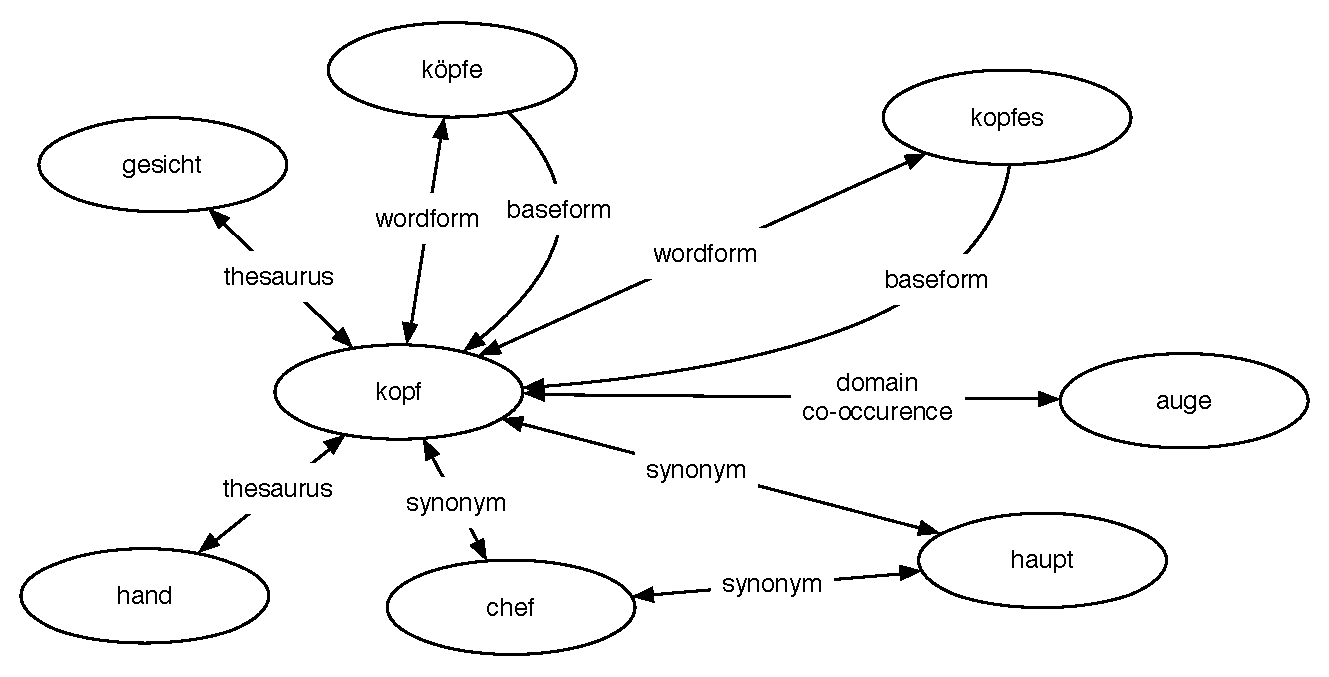
\includegraphics[width=\textwidth]{wortschatz_transformation}
\caption{Wortschatz--Daten in Graphenform}
\label{fig:wortschatz_transformation}
\end{figure}

Einen Sonderfall stellen die Kategorien der Wörter dar. Diese können in der vorliegenden Form nicht zur Link Discovery genutzt werden. Daher werden diese Daten mittels der Ermittlung von Kookkurrenzen umgeformt. Von Interesse ist, wie oft Paare von Wörtern 
in gemeinsame Kategorien eingeordnet sind. 

Somit werden bei der Transformation mittels MapReduce (siehe \cref{mapreduce_cooccurence}) Kanten mit den Kookkurrenzmaßen Dice, Jaccard und Kosinus erzeugt.

Zusammenfassend werden bei der Transformation demnach Kanten mit den Typen \emph{Synonym}, \emph{Thesaurus}, \emph{Wortform}, \emph{Grundform} und \emph{Kategorie--Kookkurrenz} erzeugt. In \cref{fig:wortschatz_transformation} wird beispielhaft ein Ausschnitt des resultierenden Graphen gezeigt. Dabei fällt auf, dass mit Ausnahme der Grundform--Kanten jede Kante in beide Richtungen existiert. Dies ist der Art der Beziehungen geschuldet, da diese in beide Richtungen gültig sind.

\subsection{Integration}

Zur Integration wird der im Transformationsschritt erzeugte Graph mit dem Zielgraphen vereinigt. Diese Vereinigung wird analog zur Integration der Clicktracking--Daten in \cref{click_integration} durchgeführt.

Insgesamt wurden dadurch \num{145023} neue Knoten und \num{50227965} neue Kanten erzeugt.  Dabei entfallen \num{48399466} Kanten auf Kookkurrenz von Kategorien, \num{550270} Kanten auf Wortformen, \num{149381} Kanten auf Grundformen, \num{279118} Kanten auf Synonyme und \num{849730} Kanten auf Thesaurus--Beziehungen.

Nachdem alle vorgenommen Schritte zur Link Discovery beschrieben wurden, beschäftigt sich der nächste Abschnitt mit einer Zusammenfassung der Ergebnisse.

\subsection{Ergebnisse}

\section{Prioisierung der Beziehungen}

Im folgenden Kapitel werden die vorgenommenen Optimierungsmaßnahmen und die damit einhergehende Evaluierung der Ergebnisse der Link Discovery beschrieben. Dazu gehören der gewählte Ansatz zur Optimierung, eine Erläuterung evolutionärer Algorithmen und deren Einsatz zur Optimierung sowie die Darstellung und Auswertung der Ergebnisse.

Zuerst muss definiert werden, welcher Aspekt genau optimiert werden soll. Die in \cref{link_discovery} beschriebenen Schritte haben einen Graphen erzeugt, in dem neun verschiedene Kantentypen existieren. Diese lauten \emph{Tag--Kookkurrenz}, \emph{Klick--Kookkurrenz}, \emph{Zusammensetzung}, \emph{Wortform}, \emph{Grundform}, \emph{Synonym}, \emph{Thesaurus--Beziehung}, \emph{Kategorie--Kookkurrenz} und \emph{Zerlegung}.

Werden nun inhaltlich relevante Nachbarn zu einem gegebenen Begriff gesucht, müssen alle ausgehenden Kanten des entsprechenden Knotens nach Relevanz geordnet werden. Dazu muss jede Kante ein Kantengewicht besitzen. Die Addition aller Kantengewichte zwischen zwei Knoten stellt somit das Maß für ihre Nähe dar.

Die Kanten vom Typ Kookkurrenz besitzen bereits aufgrund der angegebenen Kookkurrenzmaße Kantengewichte. Jedoch muss hierbei festgelegt werden, welches Maß für das Kantengewicht herangezogen werden und in welchem Verhältnis zu den Gewichten anderer Kantentypen es stehen soll.

Somit hängt die Berechnung der Relevanz zwischen zwei Knoten von zwölf Parametern ab. Jedem Kantentyp muss ein Gewicht zugewiesen und außerdem muss eine Auswahl von drei Kookkurrenzmaßen getroffen werden. Die Optimierung und Evaluierung dieser berechneten Relevanz ist Gegenstand dieses Kapitels.

Die Einschätzung, ob die Ordnung der Nachbarn eine Ordnung der Relevanz zum Ausgangsbegriff darstellt, kann nicht automatisch, sondern nur von Menschen, getroffen werden. Somit stellt die Bewertung einer bestimmten Gewichtung der Kanten auch eine Evaluierung der Kantentypen dar.
Generell kann außerdem nicht davon ausgegangen werden, dass eine einmal gefundene Gewichtung der Kanten für alle Knoten des Graphen verwertbare Ergebnisse erzeugt. Daher sollte die Optimierung nicht global, sondern für jeden Knoten einzeln erfolgen. Aufgrund der hohen Knotenanzahl wurde sich hierzu auf eine stichprobenartige Auswahl der Knotenmenge beschränkt.

Durch die Notwendigkeit menschlicher Beteiligung und der großen Anzahl an Parametern ist eine Optimierung mittels des Ausprobierens aller Fälle nicht möglich. Außerdem kann die Einschätzung, welche Kantengewichtungen relevante Ergebnisse erzeugen, stark von Mensch zu Mensch variieren. Stattdessen muss zur Optimierung ein Ansatz gefunden werden, der sich einer, für den Großteil der Personen, optimalen Gewichtung möglichst nähert. 

Im Rahmen dieser Arbeit wurde aus den genannten Gründen ein Optimierungsansatz mittels interaktiver evolutionärer Algorithmen gewählt. Die Grundlagen evolutionärer Algorithmen und die gewählte Implementierung werden in den folgenden Abschnitten beschrieben.

\subsection{Vorgehensweise}
\label{evo_implementation}

Nachdem im vorhergehenden Abschnitt die Grundlagen und Komponenten evolutionärer Algorithmen beschrieben wurden, werden im Folgenden die für die Optimierung der Link Discovery--Ergebnisse angewendeten Methoden erläutert.

Zunächst soll die Methode zur Auswahl der Stichproben erläutert werden. Insgesamt wurden fünfzehn Knoten ausgewählt, deren Beziehungen optimiert werden sollen. Die Auswahl der Knoten richtete sich nach der Popularität von Suchbegriffen auf der Website von Spreadshirt. Dazu wurden alle Begriffe mit mehr als eintausend Suchen herangezogen und diese nach Häufigkeit der Suchen geordnet. Daraus wurden zufällig je fünf Begriffe bis zum unteren Quartil, fünf Begriffe zwischen unterem und oberen Quartil und fünf Begriffe über dem oberen Quartil ausgewählt. Die ausgewählten Begriffe, deren Kantengewichtungen lokal optimiert werden sollen, lauten: \emph{Kopfkissenbezug}, \emph{Student}, \emph{Volkswagen}, \emph{Marathon}, \emph{Wow}, \emph{Krankenschwester}, \emph{Mountainbike}, \emph{Hammer}, \emph{Polska}, \emph{Regenbogen}, \emph{Minecraft}, \emph{Kind}, \emph{Dubstep}, \emph{Leipzig} und \emph{Valentinstag}.

Ziel dieser Auswahl war, eine möglichst vielfältige Verteilung der einzelnen Kantentypen zu erreichen, aus welcher sich nach Durchführung der Optimierung möglicherweise Erkenntnisse ableiten lassen, ob die Optimierung nur lokal oder auch global durchgeführt werden kann.

Nach Auswahl der Stichproben muss der Genotyp der am evolutionären Algorithmus teilnehmenden Individuen spezifiziert werden. Daraufhin muss definiert werden, wie die Komponenten des Algorithmus zu implementieren sind.

\subsection{Genotyp}

Jeder Lösungskandidat wird durch die Werte der zwölf Parameter definiert, die die Gewichtung der Kantentypen untereinander beeinflussen. Daher wird jedes Individuum als Objekt repräsentiert, dass zwölf Attribute besitzt. Davon sind neun Attribute reellwertig und drei Attribute vom Aufzählungstyp \emph{Kookkurrenzmaß}.

\begin{figure}
\centering
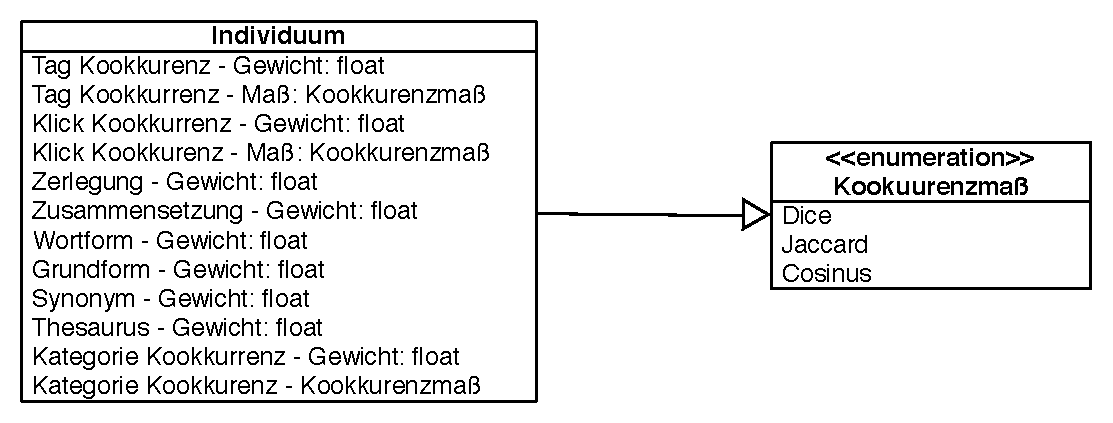
\includegraphics[width=0.9\textwidth]{genotype}
\caption{UML--Klassendiagramm des gewählten Genotyps}
\label{fig:genotype}
\end{figure}

Die reellwertigen Attribute stellen ein Gewicht des jeweiligen Kantentyps dar. Sie können nur relativ zu den anderen Kantengewichten betrachtet werden und somit nur im Rahmen der Optimierung von Interesse. Der Wertebereich dieser Attribute wird auf das Intervall \((0,1)\) eingeschränkt. Die Kookkurrenzmaße entsprechen den in \cref{measures} genannten, also \emph{Dice}, \emph{Jaccard} und \emph{Kosinus}. Der Genotyp ist in \cref{fig:genotype} als UML--Klassendiagramm und in \cref{lst:genotyope} beispielhaft in JSON--Notation dargestellt.

\begin{lstlisting}[language=json, label={lst:genotyope}, caption={Beispiel für ein Individuum}]
{
    "tagCoOccMeasure" : 0,
    "tagCoOccWeight" : 0.6878115427680314,
    "clickCoOccMeasure" : 2,
    "clickCoOccWeight" : 0.1533144270069897,
    "synonymWeight" : 0.2355003503616899,
    "thesaurusWeight" : 0.9918724503368139,
    "baseformWeight" : 0.2843543488997966,
    "wordformWeight" : 0.93317318148911,
    "sharedDomainsMeasure" : 2,
    "sharedDomainsWeight" : 0.462230023695156,
    "compositionWeight" : 0.07963851140812039,
    "decompositionWeight" : 0.4740817183628678
}
\end{lstlisting}

\subsection{Initialisierung}

Im Initialisierungsschritt wird die anfängliche Population für jede der Stichproben gebildet. Dazu muss zuerst eine geeignet erscheinende Populationsgröße festgelegt werden.

In jeder Generation müssen im Evaluierungsschritt alle Individuen bewertet werden. Wie einführend bereits erläutert wurde, kann dies nur mit menschlicher Interaktion erfolgen. Somit sollte die Populationsgröße möglichst gering sein, um mit der gleichen Anzahl Bewertungen eine größere Anzahl von Generationen zu durchlaufen. Dies geschieht auf Kosten der Diversität in der Population. Jedoch wurde im Rahmen dieser Arbeit dieser Ansatz gewählt, um möglichst viele Möglichkeiten zu haben, die Parameter zu optimieren.

Es wurde eine Populationsgröße von zehn Individuen je Stichprobe gewählt. Somit müssen in jeder Generation einhundertfünfzig Individuen bewertet werden. Bei der Initialisierung wurden die Variablen jedes erzeugten Individuums zufällig gewählt.

\subsection{Selektion}

Die Bestimmung einer Fitnessfunktion für die Optimierung der Link Discovery gestaltet sich durch die Notwendigkeit menschlicher Beurteilung als schwierig. Eine solche Fitnessbestimmung müsste derart erfolgen, dass ein Benutzer jedem Individuum einen reellwertigen Fitnesswert zuweist. Dies gestaltet ist jedoch auf Grund der hohen Anzahl von Individuen nicht praktikabel.

Die umgesetzte Selektion erfolgt durch die Durchführung von Wettkämpfen. Hierzu werden in jeder Generation je fünf Paare von Individuen gebildet. Diese Paarungen stellen die Wettkämpfe dar, bei denen der Benutzer den Gewinner bestimmt. Alle Gewinner werden selektiert und im Reproduktionsschritt weiter verwendet.

Der Vorteil dieses Vorgehens ist, dass der Benutzer nur jeweils zwei Lösungskandidaten vergleichen muss, anstatt direkt fünf der zehn Individuen auszuwählen. Somit verringert sich der zu einem Zeitpunkt zu leistende kognitive Aufwand für die Selektion.

\begin{figure}
\centering
\includegraphics[width=\textwidth]{eva_interface}
\caption{Oberfläche zur interaktiven Selektion}
\label{fig:eva_interface}
\end{figure}

Zur Selektion besucht der Benutzer eine Website, auf der ihm zwei Lösungskandidaten für eine Stichprobe präsentiert werden. Die Lösungskandidaten werden in Form von Listen von je fünfzehn Begriffen dargestellt, die die mit der jeweiligen Kantengewichtung erzeugten nächsten Nachbarn des Begriffes sind. Diese Oberfläche ist in \cref{fig:eva_interface} als Screenshot abgebildet. Nach Auswahl eines Gewinners wird dem Nutzer der nächste Wettkampf präsentiert.

Am Selektionsprozess kann sich jeder interessierte Benutzer beteiligen. Dieses Vorgehen wurde gewählt, um ein möglichst breites Spektrum an Meinungen bezüglich der Güte der Verbindungen zu erhalten.

Durch die direkte Auswahl beträgt die Reproduktionswahrscheinlichkeit für die ausgewählten Individuen eins und für die nicht ausgewählten Individuen Null \cite{sd2012}. Die gewählten Reproduktionsverfahren werden im nächsten Abschnitt beschrieben.

\subsection{Reproduktion}

Die fünf selektierten Individuen werden zur Reproduktion herangezogen, um fünf neue Individuen zu erzeugen, damit die Populationsgröße für die nächste Selektion wieder auf zehn Individuen steigt. Dazu werden die selektierten Individuen zuerst rekombiniert, um fünf Kindindividuen zu erzeugen, welche dann durch Mutation verändert werden.

\paragraph{Rekombination}

Als Verfahren zur Rekombination wurde der \emph{Ein--Punkt--Crossover} \cite{kw2007} gewählt. Dazu werden zufällig zwei Elternindividuen ausgewählt und ein zufälliger Crossover--Punkt berechnet. Werden die Genotypen der beiden Elternindividuen als Arrays dargestellt, werden bis zum Crossover--Punkt die Variablen des ersten Individuums, nach dem Crossover--Punkt die Variablen des zweiten Individuums übernommen. Der Crossover ist in \cref{fig:crossover} dargestellt.

\begin{figure}
\centering
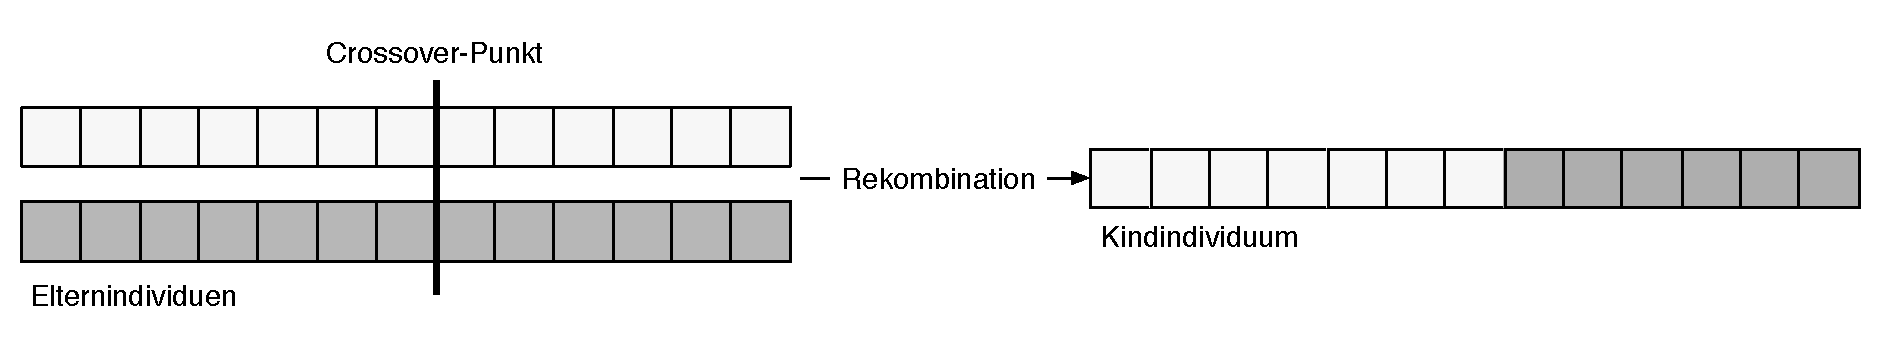
\includegraphics[width=\textwidth]{crossover}
\caption{Ein--Punkt--Crossover}
\label{fig:crossover}
\end{figure}

\paragraph{Mutation}

Zur Mutation der reellwertigen Kantengewichtungen wurde das Verfahren der \emph{Gauß-Mutation} \cite{kw2007} gewählt. Dabei wird zu jeder reellwertigen Variablen des Genotyps ein normalverteilter Zufallswert addiert. Verlässt der entstehende Wert das zulässige Intervall, so wird er auf die entsprechende Intervallschranke angepasst. Die Gauß-Mutation macht daher große Änderungen der Variable möglich, aber weniger Wahrscheinlich als kleine Änderungen. Sie eignet sich somit gut, um Diversität in der Population zu erzeugen. Konkret wurde in der Umsetzung der Optimierung eine auf das Intervall \((0,1)\) angepasste Normalverteilung mit Erwartungswert \(\mu=0\) und Varianz \(\sigma=0.5\) gewählt. Die Variablen für die Kookkurrenzmaße werden nicht mutiert.

Nachdem in diesem Abschnitt die konkrete Umsetzung der Optimierung mittels interaktiver evolutionärer Algorithmen beschrieben wurde, folgt im nächsten Abschnitt die Darstellung und Diskussion der Ergebnisse.

\subsection{Ergebnisse}

Die Optimierung wurde über insgesamt \num{13} Generationen durchgeführt. Somit wurden über alle Stichproben hinweg \num{975} Selektionen von Benutzern vorgenommen. Die Benutzer waren allesamt Mitarbeiter von Spreadshirt. Aufgrund der anonymen Teilnahme lässt sich nicht angeben, wie viele Einzelpersonen an der Optimierung teilgenommen haben.

\subsection{Kantengewichte}

Da nach jeder Selektion je Stichprobe fünf Individuen in der Population verbleiben, werden zunächst deren Kantengewichtungen untersucht. \cref{tab:winners_total} zeigt für jede Variable aus dem Genotyp den Median der in der dreizehnten Generation selektierten Individuen. Das Kantengewicht für den Typ \emph{Zerlegung} ist nicht in der Tabelle enthalten, da es sich bei den Stichproben nur um Einzelwörter handelt.

\begin{table}
\centering
\begin{tabular}{lcccccccc}
    \toprule
    Stichprobe & \(k_t\) & \(k_{kl}\) & \(s\) & \(t\) & \(g\) & \(w\) & \(k_{ka}\) & \(zu\) \\
    \midrule
    Dubstep & 0.85 & 0.60 & 0.53 & 0.77 & 1.00 & 1.00 & 1.00 & 0.48 \\
    Hammer & 0.81 & 0.56 & 0.88 & 0.45 & 1.00 & 0.89 & 0.00 & 0.59 \\
    Kind & 0.58 & 0.22 & 0.84 & 1.00 & 0.66 & 0.00 & 0.01 & 0.00 \\
    Kopfkissenbezug & 0.34 & 0.00 & 0.00 & 0.60 & 0.77 & 0.93 & 0.26 & 0.93 \\
    Krankenschwester & 1.00 & 0.20 & 0.28 & 0.60 & 0.70 & 0.88 & 0.59 & 0.33 \\
    Leipzig & 0.69 & 1.00 & 0.66 & 0.01 & 0.41 & 0.00 & 0.17 & 1.00 \\
    Marathon & 0.62 & 0.70 & 0.23 & 0.41 & 0.69 & 1.00 & 0.00 & 0.95 \\
    Minecraft & 0.71 & 0.34 & 0.31 & 0.38 & 0.74 & 1.00 & 0.00 & 1.00 \\
    Mountainbike & 0.34 & 0.48 & 0.00 & 0.00 & 1.00 & 1.00 & 0.85 & 0.00 \\
    Polska & 0.63 & 0.25 & 0.86 & 0.97 & 0.24 & 1.00 & 0.00 & 0.00 \\
    Regenbogen & 1.00 & 0.43 & 0.36 & 0.47 & 0.00 & 0.26 & 0.61 & 0.52 \\
    Student & 0.67 & 0.15 & 0.38 & 0.84 & 0.78 & 0.70 & 0.72 & 0.33 \\
    Valentinstag & 1.00 & 0.44 & 0.80 & 0.24 & 0.53 & 0.58 & 0.70 & 1.00 \\
    Volkswagen & 0.47 & 1.00 & 0.11 & 0.51 & 1.00 & 0.89 & 0.14 & 0.30 \\
    Wow & 0.08 & 1.00 & 0.93 & 0.21 & 1.00 & 0.54 & 0.53 & 0.68 \\
    \bottomrule
\end{tabular}
\caption{Mediane der Kantengewichte nach der finalen Selektion}
\caption*{
    \begin{tabular}{ll}
        \(k_t\) & Tag--Kookkurrenz\\
        \(k_{kl}\) & Klick--Kookkurrenz\\
        \(s\) & Synonyme \\
        \(t\) & Thesaurus \\
        \(g\) & Grundform \\
        \(w\) & Wortform \\
        \(k_{ka}\) & Kategorie--Kookkurrenz\\
        \(zu\) & Zusammensetzung\\
    \end{tabular}
}
\label{tab:winners_total}
\end{table}

Bei Betrachtung dieser Ergebnisse fällt auf, dass sich die Gewichtungen der Kanten von Stichprobe zu Stichprobe stark unterscheiden. Somit bestätigt sich die Vermutung, dass eine globale Optimierung der Kantengewichtungen keine sinnvollen Ergebnisse erzielt. Jedoch ergaben sich für die Typen \emph{Wortform} und \emph{Grundform} in allen Stichproben relativ hohe Gewichte.



\subsection{Kookkurrenzmaße}

In \cref{tab:measures_each} sind für alle Stichproben die nach der letzten Selektion jeweils am häufigsten in der Population auftretenden Kookkurrenzmaße aufgeführt.

\begin{table}
\centering
\begin{tabular}{llll}
    \toprule
    Stichprobe & Tags & Klicks & Kategorien \\
    \midrule
    Dubstep & Jaccard & Dice & Dice \\
    Hammer & Dice & Dice & Kosinus \\
    Kind & Kosinus & Dice & Kosinus \\
    Kopfkissenbezug & Dice & Dice & Kosinus \\
    Krankenschwester & Jaccard & Dice & Dice \\
    Leipzig & Jaccard & Jaccard & Kosinus \\
    Marathon & Dice & Dice & Jaccard \\
    Minecraft & Dice & Dice & Kosinus \\
    Mountainbike & Kosinus & Jaccard & Jaccard \\
    Polska & Jaccard & Dice & Kosinus \\
    Regenbogen & Dice & Dice & Jaccard \\
    Student & Dice & Dice & Dice \\
    Valentinstag & Dice & Jaccard & Kosinus \\
    Volkswagen & Kosinus & Dice & Dice \\
    Wow & Jaccard & Dice & Dice \\
    \bottomrule
\end{tabular}
\caption{Häufigste Kookkurrenzmaße nach der finalen Selektion}
\label{tab:measures_each}
\end{table}

\section{Zusammenfassung der Ergebnisse}

Im folgenden Abschnitt werden die quantitativen Ergebnisse der Link Discovery zusammenfassend dargestellt und diskutiert.

\begin{table}
\centering
\begin{tabular}{lrcr}
    \toprule
    Schritt & Knoten & \phantom{abc} & Kanten \\
    \midrule
    Tags & \num{314351} && \num{21834868} \\
    Clicktracking & \num{78237} && \num{310860} \\
    Zerlegung & \num{38349} && \num{1238900} \\
    Wortschatz & \num{145023} && \num{50227965} \\
    \midrule
    Gesamt & \num{575960} && \num{73612593} \\
    \bottomrule
\end{tabular}
\caption{Quantitative Ergebnisse der Link--Discovery--Schritte}
\label{tab:discovery_amounts}
\end{table}

\cref{tab:discovery_amounts} führt für jeden Schritt die hinzugefügten Knoten und Kanten sowie die nach Durchführung der Link Discovery insgesamt im Graphen enthaltene Datenmenge auf. Dabei zeigt sich, dass die Integration der Daten des Wortschatzes mit Abstand die meisten neuen Kanten in den Graphen eingefügt hat. 

Bei der Verwendung der Clicktracking--Daten wurden im Verhältnis wenig neue Knoten und Kanten erzeugt. Dies ist im Wesentlichen auf den zum Zeitpunkt des Importes noch geringen Datenbestand zurückzuführen. Daher sollte dieser Schritt zukünftig wiederholt werden, da mit der längeren Laufzeit des Clicktracking--Systems auch ein größeres Potential für neue Verknüpfungen vorhanden ist.

Neben der absoluten Anzahl der Knoten und Kanten sind bei einer Betrachtung der quantitativen Ergebnisse auch die Anzahl der Kanten, die von einem Knoten ausgehen, von Interesse. \cref{tab:discovery_edges_per_node} zeigt die Entwicklung der Kantenanzahl pro Knoten nach jedem Link--Discovery--Schritt. Dabei sind Minimum, das untere, mittlere (Median) und obere Quartil, das Maximum und der Durchschnitt dargestellt, um die Verteilung der Kantenanzahl zu verdeutlichen.

\begin{table}
\centering
\begin{tabular}{lrrrrrr}
    \toprule
    Schritt & \(min\) & \(Q_{0.25}\) & \(Q_{0.5}\) & \(Q_{0.75}\) & \(max\) & \(avg\) \\
    \midrule
    Tags & \num{0} & \num{8} & \num{15} & \num{26} & \num{35170} & \num{69,64} \\
    Clicktracking & \num{0} & \num{3} & \num{10} & \num{23} & \num{35170} & \num{56,41} \\
    Zerlegung & \num{0} & \num{4} & \num{11} & \num{24} & \num{37940} & \num{54,26} \\
    Wortschatz & \num{0} & \num{2} & \num{8} & \num{23} & \num{38380} & \num{127,8} \\
    \bottomrule
\end{tabular}
\caption{Entwicklung der Anzahl der Kanten von einem Knoten ausgehend}
\label{tab:discovery_edges_per_node}
\end{table}

Auffällig ist hierbei, dass die Integration von Clicktracking- und Wortschatz--Daten zu einer Herabsetzung des Medians führten. Dies bedeutet, dass nach Durchführung dieser Schritte verhältnismäßig weniger viel verbundene Knoten im Datenbestand existierten als davor. Jedoch deutet die Entwicklung des Durchschnittes nach der Integration der Wortschatz--Daten darauf hin, dass die Knotenanzahl viel verbundener Knoten nach diesem Schritt deutlich größer geworden ist.

Das Absinken des Durchschnittes nach Integration der Clicktracking--Daten kann in der geringen Menge der Daten begründet werden. Durch die geringe Anzahl von Kookkurrenzen konnten viel verbundene Knoten keinen relevanten Zugewinn an Verbindungen verzeichnen, während für wenig verbundene Knoten verhältnismäßig mehr neue Verbindungen hinzukamen.

Generell lässt sich festhalten, dass die Anzahl viel verbundener Knoten gemessen an der Gesamtanzahl relativ klein ist. Die Auswirkungen dessen hängen jedoch stark von der Anwendung der Daten ab und sind im Rahmen dieser Arbeit nicht beurteilbar.

Nach der quantitativen Auswertung der Link--Discovery-–Schritte wird im nächsten Kapitel die Optimierung der Kantengewichtungen und die Evaluierung der erzeugten Kanten beschrieben.
\chapter{Erstellung von Kookkurrenzgraphen}

\section{MapReduce}


\section{Anwendung von MapReduce zur Kookkurrenzberechnung}


Nachdem in diesem Kapitel die theoretischen Grundlagen für die Link Discovery mittels Kookkurrenz beschrieben wurden, beschäftigt sich das folgende Kapitel mit dem technischen System zur Umsetzung des Lösungsansatzes.
\chapter{Systembeschreibung}

Das nachfolgende Kapitel befasst sich mit der Beschreibung der Technologien und Vorgehensweisen, die zur Link Discovery im Rahmen dieser Arbeit angewendet wurden. Dazu zählen im Einzelnen die gewählte Datenbank MongoDB, das Datenmodell des Zielgraphen und das daraus resultierende Vorgehen und die Architektur des Systems zur Link Discovery.

\section{MongoDB}

Zur Umsetzung der Link Discovery wurde das Datenbankmanagementsystem MongoDB \cite{mo2013} gewählt. Bei MongoDB handelt es sich um eine quelloffene dokumentenorientierte Datenbank.

Im Gegensatz zu traditionellen relationalen Datenbanksystemen verzichtet MongoDB dabei auf eine tabellenförmige Struktur der Daten und speichert Datensätze in Form von so genannten \emph{Dokumenten}. Dabei handelt es sich um hierarchische Schlüssel-/Wertpaare, die schemalos in so genannten \emph{Collections} gespeichert werden. Schemalos bedeutet dabei, dass die Dokumente innerhalb einer Collection nicht alle dieselbe Struktur besitzen müssen.

Zur Repräsentation der Dokumente verwendet MongoDB ein Format, dass sich sehr an JSON \cite{json2006} anlehnt. JSON ist ein menschenlesbares Datenaustauschformat, das aus der Objektnotation der Programmiersprache JavaScript abgeleitet wurde. Das Datenformat von MongoDB ist BSON \cite{bson2013}, eine binäre Repräsentation von JSON, die einige zusätzliche Datentypen unterstützt. 

Listing \ref{lst:json} zeigt ein Beispiel für ein Dokument in MongoDB. Das Feld \emph{\_id} ist hierbei ein  Bezeichner vom Typ \emph{ObjectID}. Dieser stellt einen global eindeutigen Bezeichner dar, der benutzt werden kann, um Dokumente zu referenzieren. Innerhalb einer Collection ist \emph{\_id} dabei grundsätzlich eindeutig. Das Feld \emph{address} zeigt, dass Dokumente weitere Dokumente enthalten können. Das Feld \emph{friends} zeigt, dass Werte für Schlüssel auch Arrays von Werten sein können. Diese sind dabei nicht auf primitive Typen wie Zeichenketten oder Zahlen beschränkt, sondern können auch weitere Dokumente sein.

\begin{lstlisting}[language=json, label={lst:json}, caption={Ein Beispiel für ein Dokument in MongoDB}]
{
    "_id" : ObjectId("51efc20147cae77dfc02e0ac"),
    "name" : "Bob",
    "age": 25,
    "address": {
        "city": "Leipzig",
        "street": "Karl-Liebknecht-Str. 132"
        "zip": "04277"
    },
    "friends" : [
        "alice",
        "fred",
        "jason"
    ]
}
\end{lstlisting}

MongoDB unterstützt Anfragen über ein Binärprotokoll, welches über so genannte \emph{Treiber} in vielen Programmiersprachen abstrahiert zur Verfügung steht. Dabei sind vielfältige Lese- und Schreiboperationen möglich, die komplexe Abfragen und Operationen auf den gespeicherten Daten zulassen. Außerdem bietet MongoDB eine Implementierung des MapReduce-Programmiermodells (siehe \ref{mapreduce}) sowie die Möglichkeit, Indizes auf allen Hierarchieebenen der Dokumente zu nutzen. Für interaktive Operationen steht die \emph{Mongo Shell} zur Verfügung, welche Abfragen mittels der Programmiersprache JavaScript erlaubt und somit einen Treiber für diese Sprache darstellt.

Aufgrund der genannten Eigenschaften stellt MongoDB einen exzellenten Ausgangspunkt für die Link Discovery im Rahmen dieser Arbeit dar. Durch die vorhandene Schemaflexibilität können die Daten in der gerade benötigten Form gespeichert und abgefragt werden. Durch die Unterstützung von MapReduce mit mehreren Rechnern lassen sich Berechnungen wie die der Kookkurenz (siehe \ref{mapreduce_cooccurence}) parallelisieren und somit beschleunigen.

Aus diesen Gründen stellt MongoDB das zentrale technische Element für die Link Discovery im Rahmen dieser Arbeit dar. Sobald die Daten aus den externen und internen Quellen in MongoDB importiert wurden, können die folgenden Schritte direkt mit Datenbankabfragen realisiert werden.

\section{Datenmodell}

Nach der Auswahl eines geeigneten Datenbanksystems sollte das Datenmodell des Ergebnisses genauer spezifiziert werden. Ist dieses vor der Link Discovery klar, können die einzelnen benötigten Schritte zur Erreichung des Zieles einfacher definiert werden.

Generell handelt es sich bei dem gewünschten Ergebnis um einen gerichteten Multigraph. Dieser repräsentiert Objekte, oder auch \emph{Knoten}, zwischen denen paarweise Verbindungen, die \emph{Kanten} bestehen. Die Besonderheit eines Multigraphen ist dabei, dass zwischen zwei Knoten auch mehrere Kanten existieren dürfen \cite{rd2012}. Dies ist dem gewählten Lösungsansatz geschuldet, da zwischen Wörtern und Wortgruppen verschiedenartige Beziehungen existieren können.

Somit müssen für das Datenmodell die beiden Entitäten \emph{Knoten} und \emph{Kante} modelliert werden.

\subsection{Knoten}

Die Knoten repräsentierendie Wörter und Wortgruppen zwischen denen durch Link Discovery Verbindungen hergestellt werden sollen. Sie enthalten als benötigte Attribute eine Zeichenkette und ein Attribut Sprache. Die Kombination dieser beiden Attribute ist innerhalb der Knotenmenge eindeutig. Außerdem erhält jeder Knoten zur einfacheren Referenzierung einen eindeutigen Bezeichner.

Neben diesen immer vorhandenen Attributen kann ein Knoten beliebig viele weitere Eigenschaften besitzen. Diese Eigenschaften dienen dazu, den Begriffen, die die Knoten existieren, für spätere Verwendungen zusätzlichen Kontext zu geben. Im Wesentlichen definieren sich diese zusätzlichen Eigenschaften aus den Datenquellen, die zum Zweck der Link Discovery in den Graph integriert werden.

Zur besseren Kapselung und Übersicht sollten die zusätzlichen Eigenschaften in weitere Entitäten gekapselt werden. Die Struktur dieser zusätzlichen Typen kann dann zum Zeitpunkt der Integration der jeweiligen Datenquelle definiert werden.

Das resultierende Knotenmodell ist in Abbildung \ref{fig:node_erd} dargestellt.

\begin{figure}
\label{fig:node_erd}
\begin{center}
    \includegraphics[width=0.6\textwidth]{node_erd}
\end{center}
\caption{Knotenmodell als Entity-Relationship-Diagramm}
\end{figure}

\subsection{Kanten}



\subsection{Technische Umsetzung}

\begin{figure}
\label{fig:graph_model}
\begin{center}
    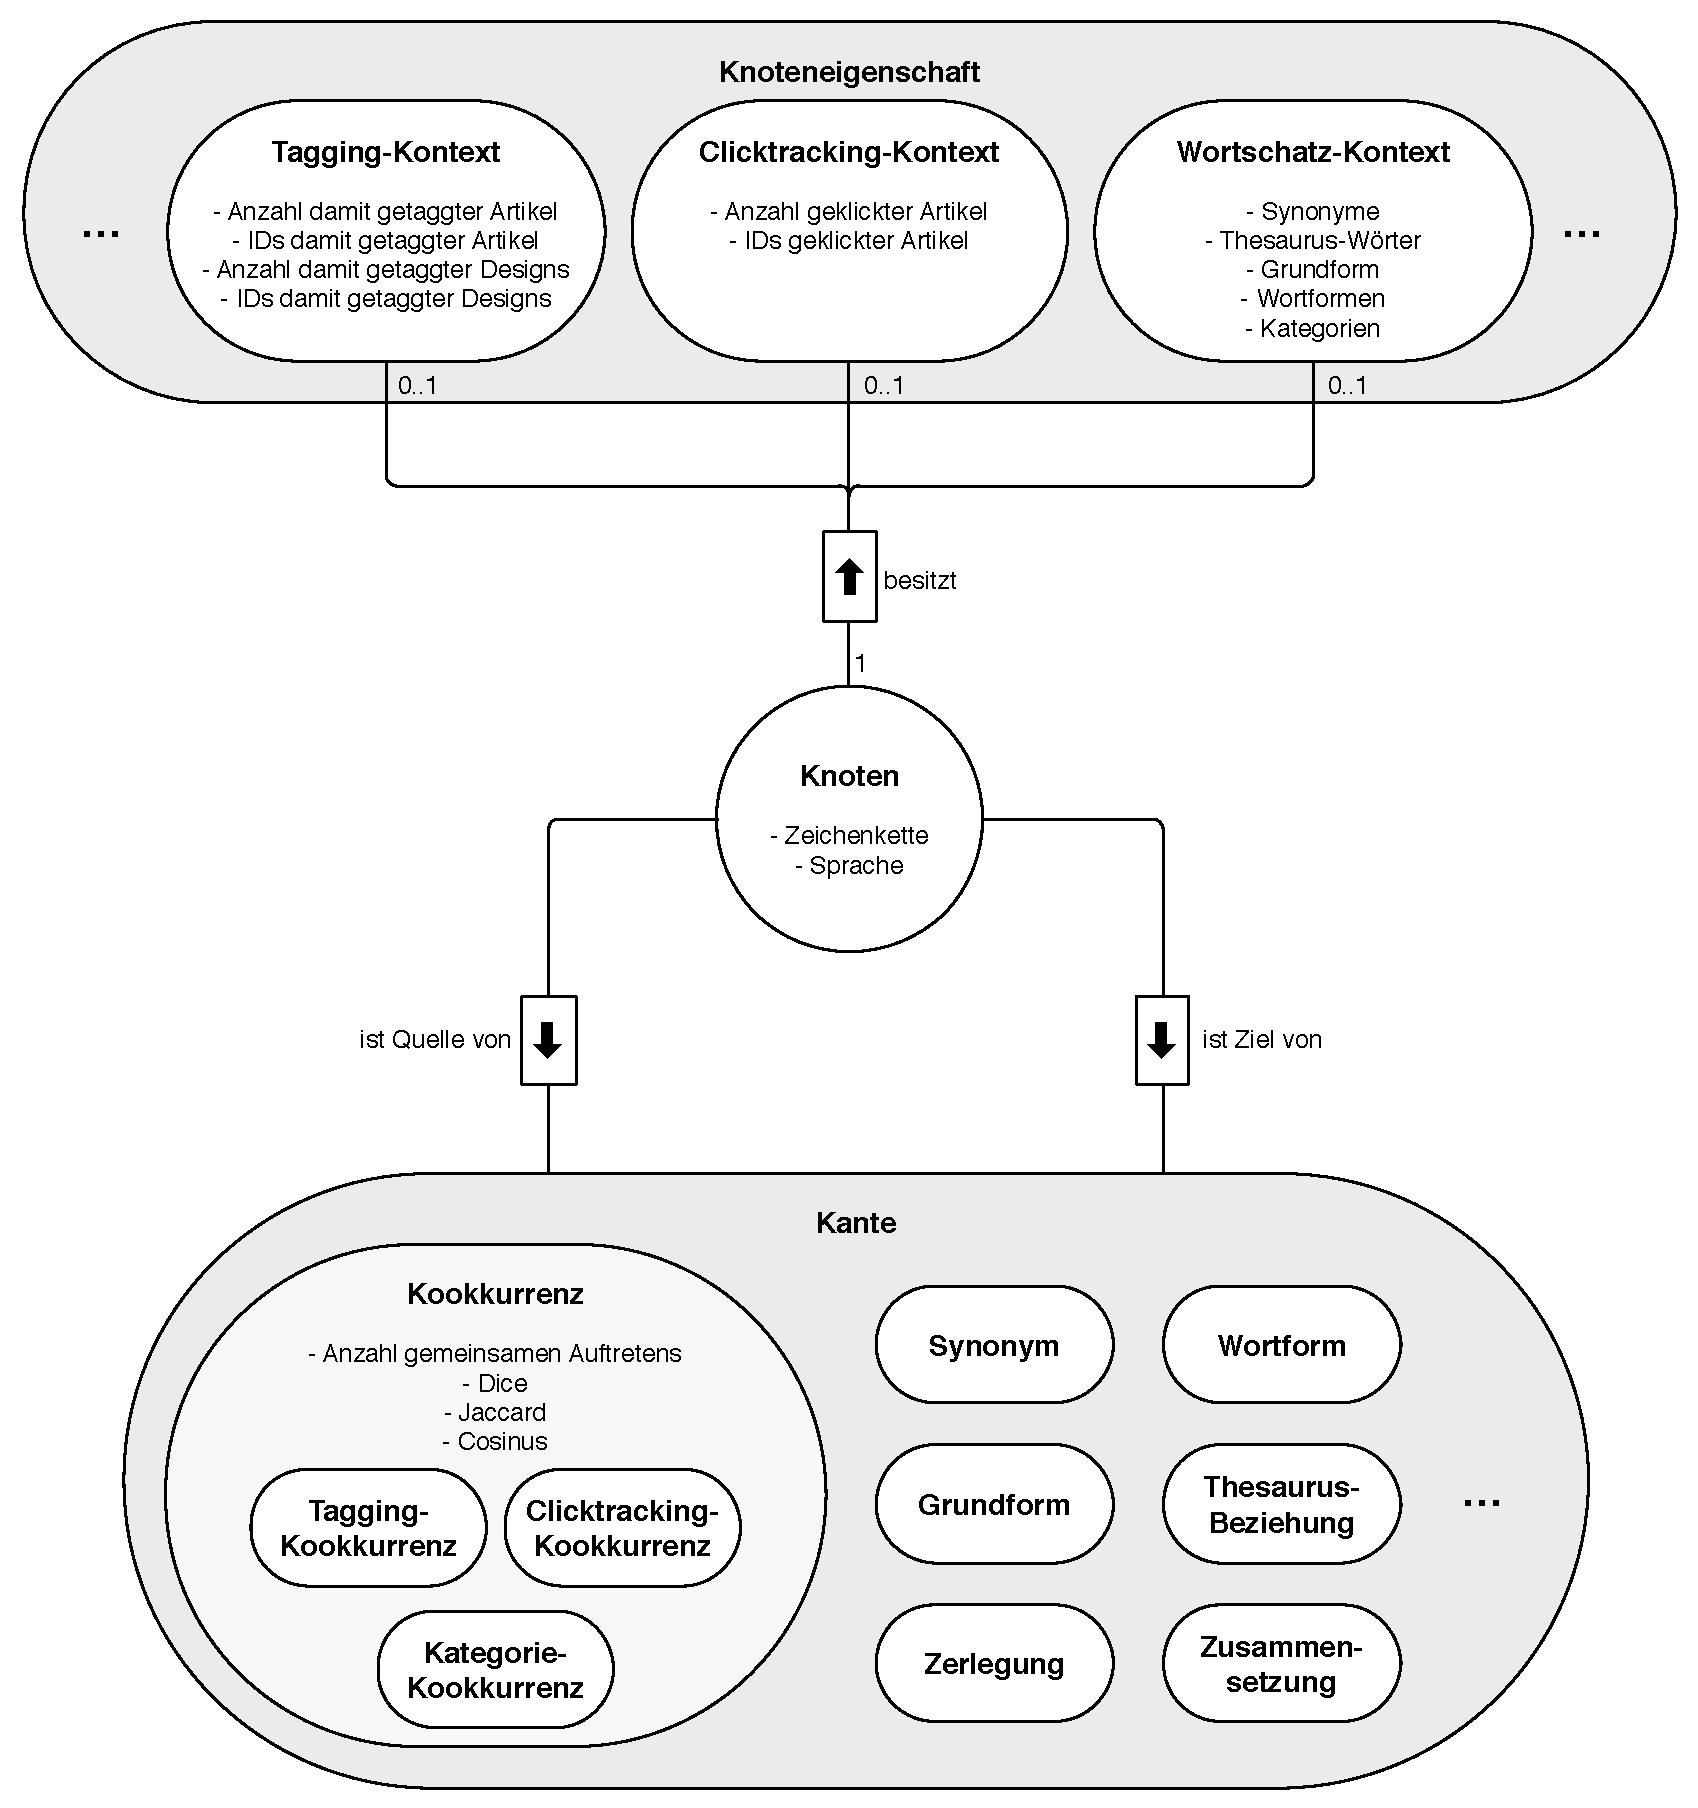
\includegraphics[width=1\textwidth]{graph_model}
\end{center}
\caption{Datenmodell des Graphen als Entity-Relationship-Diagramm}
\end{figure}

\section{Systemarchitektur}

\begin{figure}
\label{fig:architecture}
\begin{center}
    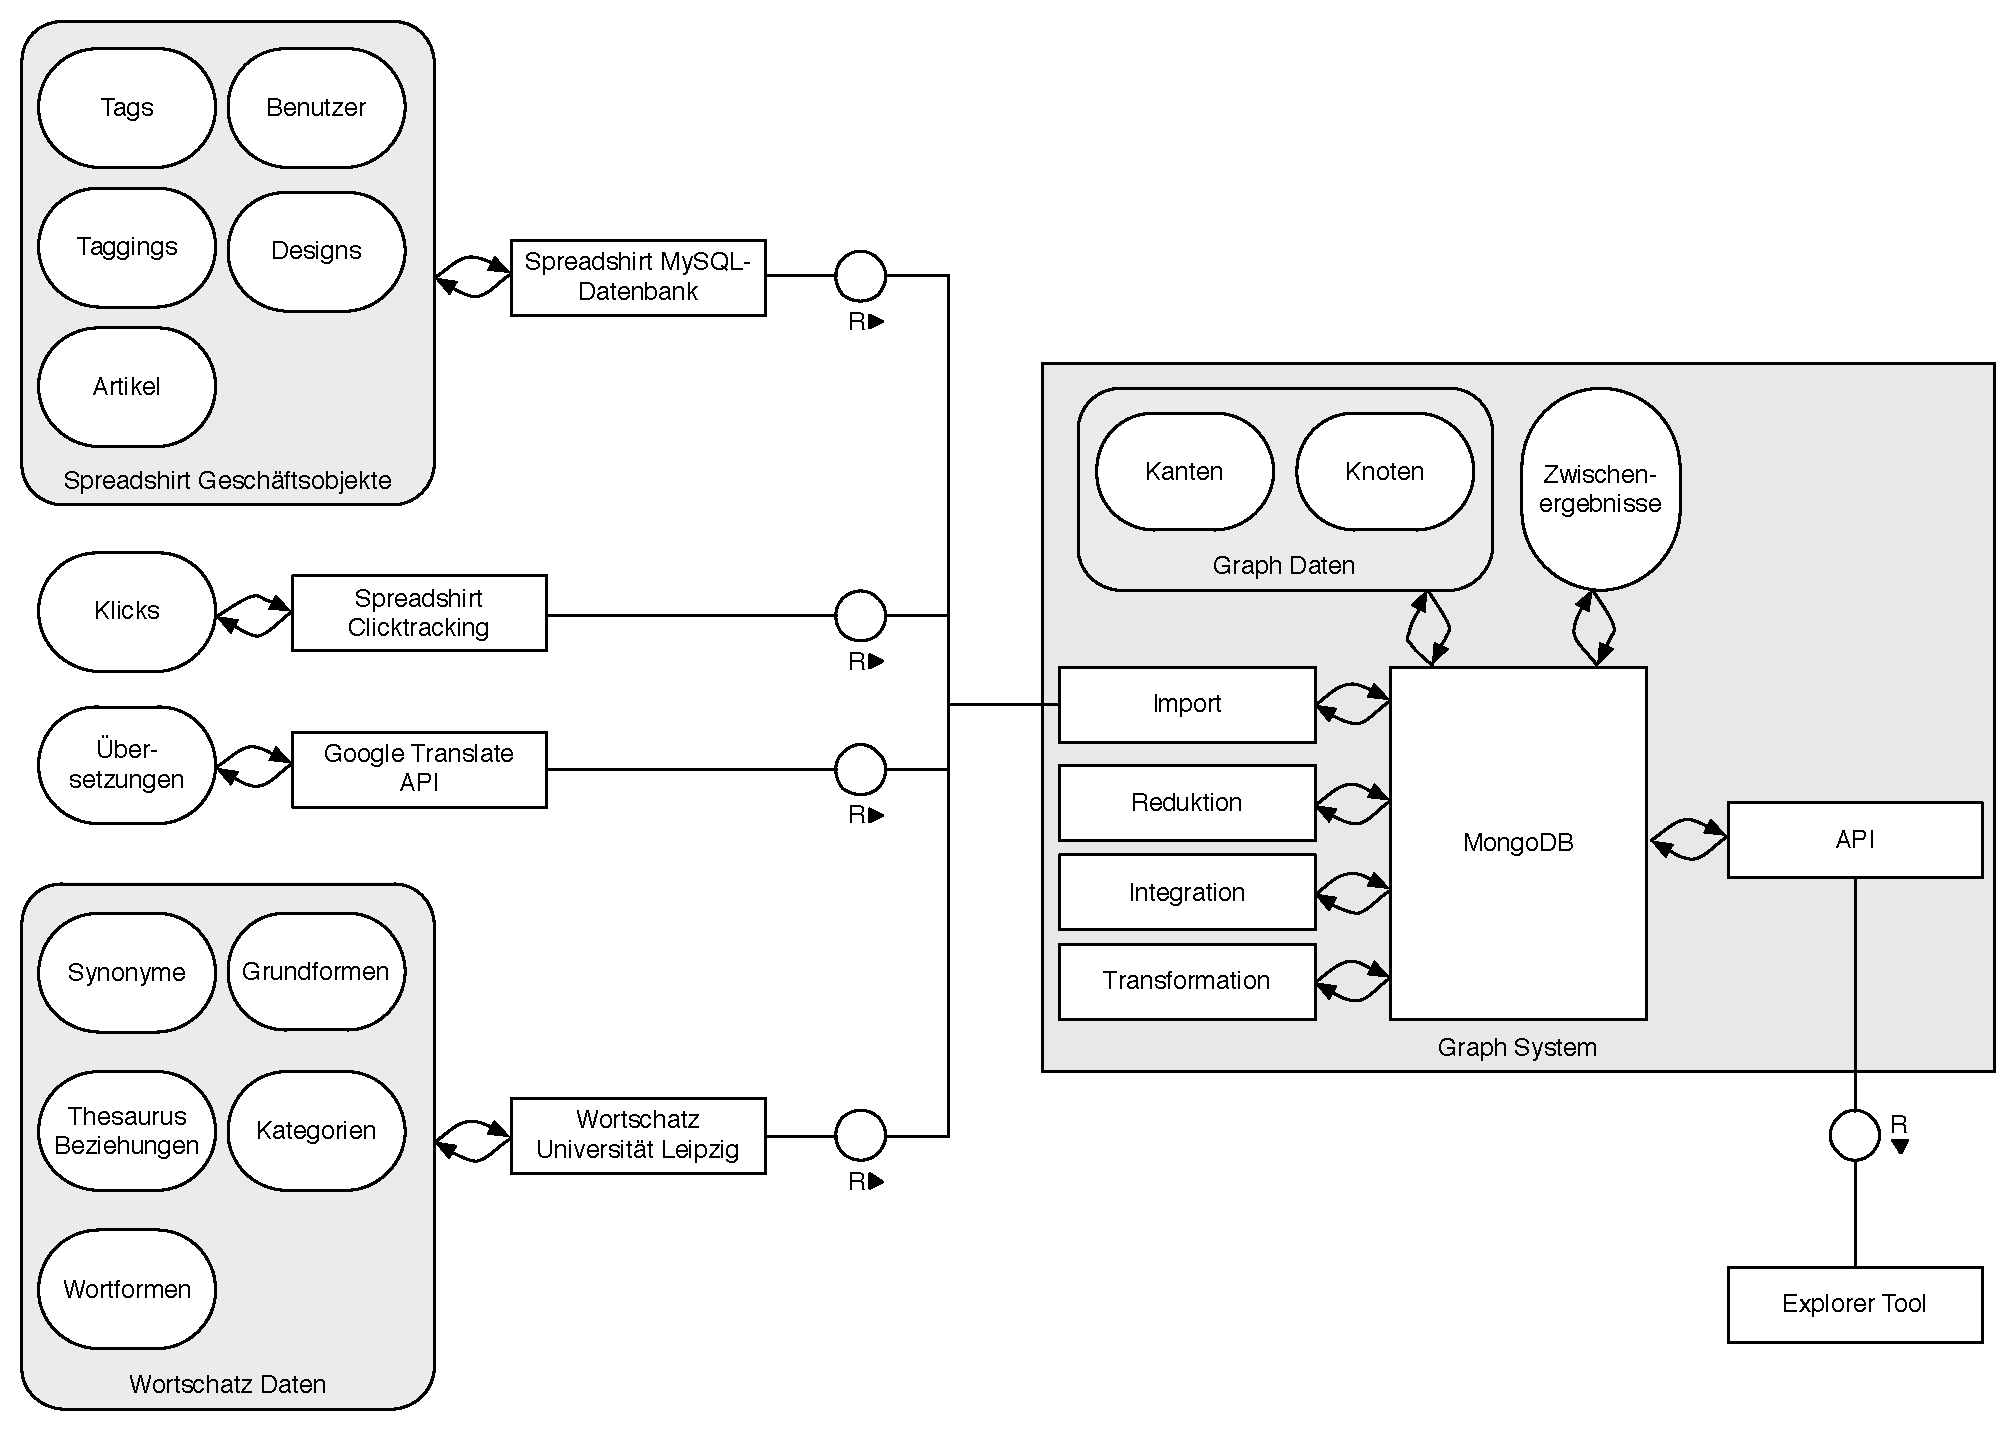
\includegraphics[width=1\textwidth]{architecture}
\end{center}
\caption{Systemarchitektur}
\end{figure}

\chapter{Schlussbetrachtung}
\label{summary}

\section{Fazit}

\section{Ausblick}

\listoffigures
\listoftables
\lstlistoflistings

\sloppy
\printbibliography 

\end{document}